% MCM/ICM 2025 C题 终稿
% 编译器：xelatex
\documentclass{mcm-paper}

% 常用数学宏
% 跨文档共享

% 数域
\newcommand{\R}{\mathbb{R}}
\newcommand{\N}{\mathbb{N}}
\newcommand{\Z}{\mathbb{Z}}
\newcommand{\C}{\mathbb{C}}

% 统计
\newcommand{\E}{\mathbb{E}}
\newcommand{\Var}{\operatorname{Var}}
\newcommand{\Cov}{\operatorname{Cov}}

% 优化
\newcommand{\minimize}{\operatorname{minimize}}
\newcommand{\subjectto}{\text{subject to}}

% 微积分
\newcommand{\pd}[2]{\frac{\partial #1}{\partial #2}}
\newcommand{\norm}[1]{\left\lVert #1 \right\rVert}


% 补充包
\usepackage{float}
\usepackage{xcolor}
\usepackage{tikz}
\usetikzlibrary{arrows.meta, positioning, shapes.geometric, calc, backgrounds}

% 图表路径
\graphicspath{{../artifacts/figures-body/}{../artifacts/figures-appendix/}}

% 参考文献
\addbibresource{../../../../../references/bib/references.bib}

% --- 标题页信息 ---
\title{NIPT 最佳时点选择与胎儿染色体异常筛查的数学模型}
\date{2025年7月19日}

\begin{document}

% ============================================================
% SUMMARY SHEET（独立首页，不计页数，≤300 词）
% ============================================================
\begin{center}
{\Large\bfseries 摘要}
\end{center}

\vspace{0.5em}

无创产前检测（NIPT）通过母体外周血中胎儿游离 DNA 筛查染色体非整倍体。其可靠性取决于胎儿 DNA 浓度（Y 染色体浓度 $\geq 4\%$），而浓度受孕周、BMI 等多种因素影响。本文围绕两个核心问题建模：（1）何时进行 NIPT 可使检测不可靠的风险最小？（2）如何利用 Z 值以外信息判定女胎染色体异常？

针对问题 1，利用 267 位男胎孕妇的纵向检测数据，发现横向 Spearman 相关近零（Y$\sim$孕周 $\rho=0.084$）的原因是 65\% 的变异来自个体基线差异。采用个体内中心化回归模型剥离基线后，孕周效应 $\hat{\beta}_1=+0.055$（每周 $+5.7\%$，$p<0.001$），BMI 负效应 $\hat{\beta}_2=-0.029$（$p<0.001$），中介分析表明 21\% 的孕周效应通过胎儿 DNA 总量增加间接实现。留一孕妇交叉验证 $R^2_{\mathrm{CV}}=0.248$，HC3 稳健标准误验证所有结论不受异方差影响。

针对问题 2 和 3，基于「补测不消耗不可逆临床窗口期」的非对称代价逻辑，提出 $p_0=0.5$ 的直接计数策略确定各组最佳 NIPT 时点。BMI $[28,32)$ 组推荐 11 周（达标率 94\%，Wilson 95\% CI $[74\%,99\%]$），$[32,36)$ 组推荐 12 周（达标率 86\%，CI $[71\%,92\%]$），$[36,40)$ 组推荐 14 周（达标率 75\%），BMI $\geq 40$ 组采用两阶段策略（14 周预检 $+$ 18--20 周复检）。多因素回归排除了年龄、怀孕次数等额外因素（$p>0.6$），$p_0$ 灵敏度分析显示 88\% 人群的推荐时点在 $p_0=0.4\sim0.8$ 范围内完全不变。

针对问题 4，面对经典 $Z>3$ 规则召回率仅 4.5\% 的困境，利用 GC bias 校正（loess）和 Tikhonov 正则化 Fisher 线性判别分析，按染色体拆分判别器（13/18/21 号），以测序质控指标和染色体特异性 GC 差异为主特征。高灵敏度策略（TPR$\geq 90\%$）实现召回率 93.8\%（AUC=0.775），仅漏检 1 人，低风险组安全性 96.2\%。

本文贡献在于：（1）揭示了纵向数据结构中个体基线的主导地位，为群体均值回归的失效提供了方法论解释；（2）建立了以直接计数替代外推预测的保守策略，避免小样本尾部风险；（3）在 Z 值信号意外缺位的约束下，发现了测序质控指标和 GC 跨染色体差异的替代判别路径。

\vspace{1em}
\noindent{\bfseries 关键词：}NIPT；胎儿游离 DNA；个体内中心化；BMI 分组；Fisher 线性判别；GC 校正

\newpage

% ============================================================
% TABLE OF CONTENTS
% ============================================================
\tableofcontents
\newpage

% ============================================================
% 1. INTRODUCTION
% ============================================================
\section{引言}

\subsection{问题背景}

无创产前检测（NIPT）通过分析母体外周血中的胎儿游离 DNA（cfDNA）筛查常见染色体非整倍体（T21、T18、T13）。自 Lo 等人 1997 年首次发现母体血浆中存在胎儿 DNA 以来\cite{lo1997}，NIPT 已成为产前筛查的标准工具。检测可靠性的核心前提是胎儿 cfDNA 在总游离 DNA 中达到足够比例——临床上通常以 Y 染色体浓度 $\geq 4\%$ 作为男胎 NIPT 结果可靠的标准。

然而，胎儿 cfDNA 浓度受多种因素影响。Wang 等人在 22,384 例大样本中证实\cite{wang2013}：cfDNA 占比随孕周缓慢上升，但与母体体重显著负相关。对于以高 BMI 人群为主的检测群体，达标时间可能显著延后，而过晚检测（$\geq 28$ 周）将导致治疗窗口关闭。

此外，对于女胎，Y 染色体浓度无法作为 cfDNA 浓度的代理指标。临床上依赖 Z 值判断染色体拷贝数异常，但 Z 值可能受测序 GC 偏差、限制性胎盘嵌合体（CPM）\cite{grati2014}等因素干扰。如何利用 Z 值以外的信息维度判定异常，是女胎筛查的核心难题。

\textbf{本工作的方法论立场}：我们处理的是回顾性临床数据而非受控实验，因此所有回归系数均解读为统计关联而非因果效应。但模型的输出——BMI 分组与检测时点——最终需要转化为可执行的临床建议。为此，全文的时点建议均以整周给出：这一选择并非出于计算简化，而是因为产前检测的预约体系和孕周估算均以整周为基本单位，小数孕周建议在实际操作中缺乏对应的时间锚点。

\subsection{本文工作}

本文围绕 2025 年全国大学生数学建模竞赛 C 题，解决四个子问题：

\begin{enumerate}
    \item \textbf{Y 染色体浓度建模}：利用 267 位男胎孕妇的纵向数据，建立 Y 浓度与孕周、BMI 的关系模型，检验显著性。
    \item \textbf{BMI 分组与最佳 NIPT 时点}：基于非对称代价逻辑，按 BMI 分组给出各组最佳检测时点。
    \item \textbf{多因素验证}：穷举检验所有候选因素，验证问题 2 分组的稳健性。
    \item \textbf{女胎异常判定}：在 Z 值信号缺位的约束下，构建基于 GC 含量和测序质控的异常判定方法。
\end{enumerate}

子问题 1--3 构成男胎路径（Y 浓度建模 $\to$ 达标预测 $\to$ 分组与时点），子问题 4 为独立的女胎路径。整体架构如图~\ref{fig:arch}所示。

\begin{figure}[H]
\centering
\begin{tikzpicture}[
    box/.style={draw, rounded corners=3pt, minimum width=2.8cm, minimum height=0.7cm, align=center, font=\small\sffamily},
    subbox/.style={draw, rounded corners=2pt, minimum width=2.2cm, minimum height=0.7cm, align=center, font=\footnotesize\sffamily},
    data/.style={fill=blue!8, draw=blue!40},
    model/.style={fill=orange!8, draw=orange!50},
    output/.style={fill=green!8, draw=green!50},
    arrow/.style={-{Stealth[scale=0.8]}, line width=0.6pt, draw=gray},
    darrow/.style={-{Stealth[scale=0.7]}, dashed, line width=0.5pt, draw=gray!60},
]

% ===== 数据层 =====
\node[box, data, minimum width=7cm] (raw) at (0,0)
    {原始数据（男胎 1082 条 + 女胎 605 条）};

% ===== 男胎路径 =====
\node[box, model] (sub1) at (-2.5,-1.6) {子问题 1\\Y 浓度建模};
\node[subbox, output] (out1) at (-2.5,-2.7) {$\hat{\beta}_1$: 孕周 $+5.7\%$/周\\$\hat{\beta}_2$: BMI $-3\%$/单位};
\node[box, model] (sub2) at (-2.5,-3.9) {子问题 2\\BMI 分组与最佳时点};
\node[subbox, output] (out2) at (-2.5,-5.0) {三组方案：\\11--12 / 14 / 两阶段};
\node[box, model] (sub3) at (-2.5,-6.2) {子问题 3\\多因素验证};
\node[subbox, output, minimum height=0.5cm] (out3) at (-2.5,-7.1) {分组方案不变，独立验证通过};

\draw[arrow] (raw.south) -- ++(0,-0.2) -| (sub1.north);
\draw[arrow] (sub1.south) -- (out1.north);
\draw[arrow] (out1.south) -- (sub2.north);
\draw[arrow] (sub2.south) -- (out2.north);
\draw[arrow] (out2.south) -- (sub3.north);
\draw[arrow] (sub3.south) -- (out3.north);

% ===== 女胎路径 =====
\node[box, model] (sub4) at (2.5,-1.6) {子问题 4\\女胎异常判定};
\node[subbox, output] (out4) at (2.5,-2.7) {召回率 $93.8\%$\\低风险安全性 $96.2\%$};

\draw[arrow] (raw.south) -- ++(0,-0.2) -| (sub4.north);
\draw[arrow] (sub4.south) -- (out4.north);

% ===== 横向连接 =====
\draw[darrow] (-1.1,-1.6) -- node[above, font=\tiny\color{gray}]{测序质控方法} (1.1,-1.6);

% ===== 标签 =====
\node[font=\small\bfseries, blue!60!black] at (-2.5, 0.45) {男胎路径};
\node[font=\small\bfseries, red!60!black]  at (2.5, 0.45)  {女胎路径};

% ===== 方法标注 =====
\node[font=\footnotesize\color{gray}, anchor=west] at (2.5,-4.2)
    {GC校正 $\to$ Fisher LDA};

\end{tikzpicture}
\caption{跨子问题模型架构}
\label{fig:arch}
\end{figure}

\newpage

% ============================================================
% 2. ASSUMPTIONS
% ============================================================
\section{模型假设}

\begin{enumerate}
    \item \textbf{条件对数正态性}：Y 染色体浓度经对数变换后，在给定协变量条件下残差近似正态。原始 Y 浓度偏度 0.70（Shapiro-Wilk $W=0.90, p<10^{-16}$），$\ln(Y)$ 后偏度降至 $-0.55$（Shapiro-Wilk $W=0.995, p=0.11$），模型残差 $W=0.997$（$p=0.41$）。对数变换使数据在 5\% 显著性水平上不拒绝正态性假设。
    \item \textbf{个体内线性孕周效应}：同一孕妇内 Y 浓度对数随孕周线性增长。留一孕妇交叉验证中，线性形式的预测精度显著优于三次样条和指数形式（Wilcoxon $p<0.001$）。
    \item \textbf{月份批次效应可加}：2023 年 9--12 月 Y 浓度系统性偏低的批次效应为固定偏移，不与孕周或 BMI 交互。加入月份哑变量后 CV $R^2$ 从 0.138 升至 0.229，模型未因该假设退化。
    \item \textbf{GC 偏差在比值中约消}：Y 浓度 = Y reads / 总 reads，总体 GC 含量对分子和分母产生同向影响。实证：GC 正常组与偏低组的 Y 浓度达标率曲线重合（组间差 $<2$ 个百分点），GC 含量在回归中 $t=1.34, p=0.18$。
    \item \textbf{Fisher LDA 线性可分性}：经 GC 校正和 Tikhonov 正则化后，正常与异常样本在所选特征空间中线性可分。AUC=0.775 表明存在中等程度的可分性。受限于阳性样本仅 12 例（去重后），无法对非线性方法（如核 LDA、SVM）做有统计效力的对比——但方案对比验证（见表~\ref{tab:perf}）确认 Fisher LDA 在简单替代方案中为最优。
    \item \textbf{回顾性数据的关联解释}：本数据为回顾性临床数据，检测时点非随机（可能存在 indication bias）。报告中的回归系数解读为统计关联而非因果效应。
\end{enumerate}

% ============================================================
% 3. NOTATIONS
% ============================================================
\section{符号说明}

\begin{table}[H]
\centering
\caption{主要符号表}
\begin{tabular}{ll}
\toprule
符号 & 含义 \\
\midrule
$y_{it}$ & 孕妇 $i$ 第 $t$ 次检测的 Y 染色体浓度 \\
$g_{it}$ & 孕妇 $i$ 第 $t$ 次检测时的孕周（周） \\
$\Delta g_{it}$ & 个体内中心化孕周：$g_{it}-\bar{g}_i$ \\
$\mathrm{BMI}_i^*$ & 中心化 BMI \\
$p_0$ & 达标把握阈值 \\
$t^*$ & 推荐 NIPT 时点 \\
$\tilde{z}_i^{(k)}$ & 第 $k$ 号染色体 GC 校正后 Z 值 \\
$\mathbf{S}_W^{(k)}$ & 第 $k$ 号染色体判别器的类内散度矩阵 \\
$\mathbf{w}^{(k)}$ & Fisher LDA 判别权重向量 \\
$\tau^*$ & 高灵敏度阈值（TPR $\geq 90\%$） \\
\bottomrule
\end{tabular}
\end{table}

% ============================================================
% 4. MODELS
% ============================================================
\section{模型构建}

\subsection{子问题 1：Y 染色体浓度建模}

\subsubsection{核心难点：横向信号被个体基线淹没}

男胎数据包含 267 位孕妇的 1082 条纵向检测记录（多数每人 4 次，时间跨度 10--25 周）。初步探索揭示了一个结构性困难：Y 浓度与孕周的横向 Spearman 相关系数仅 $\rho=0.084$（可忽略），与 BMI 仅 $\rho=-0.155$。这并非因为没有效应——而是不同孕妇的 Y 浓度基线差异可达 3--4 倍，个体间基线差异（占总变异约 65\%）完全淹没了群体层面的孕周或 BMI 趋势。

这意味着横截面回归将一无所获。必须利用数据的纵向结构——剥离个体基线后，在同一孕妇内部观察 Y 浓度的变化规律。

\subsubsection{个体内中心化回归}

将 Y 浓度取对数（$\tilde{y}_{it}=\ln y_{it}$）以满足正态性假设，构建个体内中心化回归：

\begin{equation}
\tilde{y}_{it} = \beta_0 + \beta_1 \Delta g_{it} + \beta_2 \mathrm{BMI}_i^* + \sum_{k=1}^{4} \theta_k \mathrm{Tech}_{it}^{(k)} + \sum_{m=1}^{16} \gamma_m \mathrm{Month}_m^{(it)} + \varepsilon_{it}
\label{eq:modelA}
\end{equation}

其中 $\mathrm{Tech}^{(1\sim4)}$ 为四项测序质控指标（原始读段数、比对比例、重复读段比例、过滤比例），$\mathrm{Month}_m$ 为月份哑变量。

\subsubsection{参数估计}

表~\ref{tab:coef-main} 报告核心系数。孕周（个体内）$\hat{\beta}_1=+0.055$（$t=13.96, p<0.001$），每周 Y 浓度增加约 $e^{0.055}\approx 5.7\%$。BMI $\hat{\beta}_2=-0.029$（$t=-6.97, p<0.001$），BMI 每高 1 单位，Y 浓度降约 3\%。

全模型 $R^2=0.294$，留一孕妇 CV $R^2_{\mathrm{CV}}=0.248$。效应量分解：个体间基线差异 65\%，孕周直接贡献 10\%，BMI 约 5\%，技术+批次共约 10\%。

\begin{table}[H]
\centering
\caption{模型 A 核心系数}
\label{tab:coef-main}
\begin{tabular}{lrrr}
\toprule
变量 & 估计值 & $t$ 值 & $p$ 值 \\
\midrule
孕周（个体内） & $+0.055$ & 13.96 & $<0.001$ \\
BMI（中心化）  & $-0.029$ & $-6.97$ & $<0.001$ \\
过滤比例       & —      & 3.68   & $<0.001$ \\
读段数         & —      & $-4.54$ & $<0.001$ \\
重复读段比例   & —      & 2.44   & 0.015 \\
\bottomrule
\multicolumn{4}{l}{\footnotesize 全模型 $R^2=0.294$, CV $R^2=0.248$。月份批次系数从略。} \\
\end{tabular}
\end{table}

模型诊断：残差近似正态，异方差轻微（低拟合区 SD=0.46 vs 高区 SD=0.34），但 HC3 稳健标准误验证显示最大膨胀比仅 1.255（BMI），所有变量仍高度显著（$|t|>2.6$），对推断无实质影响。

\begin{figure}[H]
\centering
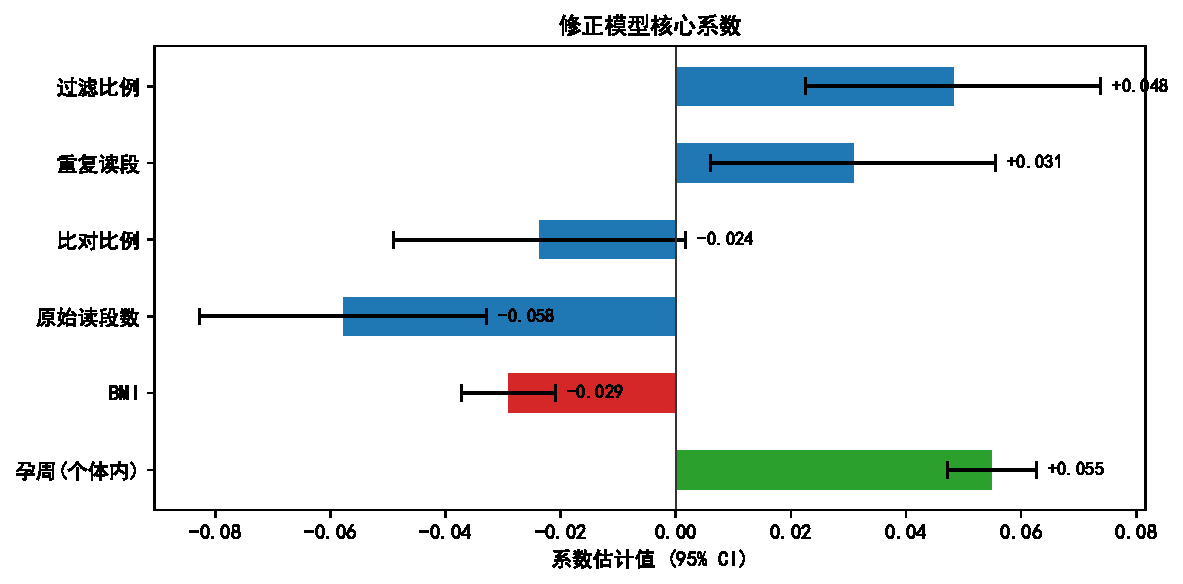
\includegraphics[width=0.7\textwidth]{sub1-final-coefficients.pdf}
\caption{核心系数估计及 95\% 置信区间}
\label{fig:coef}
\end{figure}

\subsubsection{中介分析}

模型 B 加入 X 染色体浓度（与 Y 同源，反映胎儿 DNA 总浓度）探索效应传递路径：

\begin{equation}
\tilde{y}_{it} = \beta_0' + \beta_1' \Delta g_{it} + \beta_2' \mathrm{BMI}_i^* + \beta_X' X_{it}^* + \text{controls} + \varepsilon_{it}'
\end{equation}

加入 X 后，孕周系数从 $+0.055$ 降至 $+0.045$（下降 21.3\%），BMI 系数几乎不变（$-0.029\to -0.023$）。以孕妇为单位的 Bootstrap（$B=1000$）给出中介比例的 95\% 置信区间为 $[14.9\%, 27.3\%]$，区间不含零且在合理范围内——21\% 的孕周效应通过「胎儿发育 $\to$ DNA 总量增加」间接实现；BMI 的负效应与此通路在统计上独立，与文献记载的血浆体积稀释机制一致\cite{wang2013}。全样本 $R^2$ 提升至 $0.441$。

\begin{figure}[H]
\centering
\begin{tikzpicture}[
    node distance=2.2cm and 2.5cm,
    box/.style={draw, rounded corners=3pt, minimum width=3.5cm, minimum height=0.7cm,
                align=center, font=\small\sffamily, fill=orange!6},
    arrow/.style={-{Stealth[scale=0.9]}, line width=1pt},
    label/.style={font=\footnotesize\color{gray}, fill=white, inner sep=1pt},
]

\node[box] (gw) at (0,0) {孕周};
\node[box] (x)  at (0,-2.5) {X 染色体浓度\\（胎儿 DNA 总量）};
\node[box] (y)  at (5,0) {Y 染色体浓度};

% c': direct effect
\draw[arrow] (gw.east) -- node[above, label] {$c' = +0.045^{***}$} (y.west);

% a: path from gw to X
\draw[arrow] (gw.south) -- node[left, label, pos=0.45] {$a$} (x.north);

% b: path from X to Y
\draw[arrow] (x.east) -| node[below, label, pos=0.7] {$b = +4.817^{***}$} (y.south);

% Total = c' + a*b
\node[font=\footnotesize, anchor=north] at (5,-4.0)
    {总效应 $c = c' + a \times b = +0.055^{***}$};
\node[font=\footnotesize, anchor=north] at (5,-4.5)
    {中介比例 $= (c-c')/c \approx 21.3\%$};

\end{tikzpicture}
\caption{孕周 $\to$ Y 浓度的中介效应路径。孕周通过两条路径影响 Y 浓度：直接路径 $c'$ 和经 X 染色体浓度的间接路径 $a\times b$。}
\label{fig:med}
\end{figure}

\subsection{子问题 2：BMI 分组与最佳 NIPT 时点}

\subsubsection{非对称代价与策略框架}

问题的关键在于代价结构的不对称：测太早（Y $<4\%$）导致检测结果不可靠，但补测不消耗不可逆的临床窗口期；测太晚（$\geq 28$ 周）导致治疗窗口关闭，不可逆。传统的「两种风险加权求和」范式在此不适用——正确策略是\textbf{在可接受的达标把握下，尽可能早测}。

治疗窗口采用三阶梯风险：$\leq 12$ 周（低风险）、13--27 周（高风险）、$\geq 28$ 周（极高风险）。所有建议时点均不超过 25 周。补测虽产生额外经济支出（NIPT 单次检测约 1,000--3,000 元/次），但与错过治疗窗口的不可逆后果相比，仍在可接受范围内。

全文时点建议以整周给出而非小数孕周，是基于临床可操作性：小数孕周建议（如 12.4 周）不符合实际医患交流情形，无法指导实践。仅当数据允许时以半周精度进行灵敏度检验，最终建议均舍入至整周。

\subsubsection{前提验证}

对 260 位有首次达标记录的孕妇做多元回归：体重（标准系数 $+0.576$, $p<0.001$）和 BMI（$+0.438$, $p=0.008$）是仅有显著贡献的变量。年龄（$p=0.39$）、IVF 状况（$p=0.08$）均不显著。BMI 独自解释了达标时间变异的主要部分——题目前提得到数据支持。

\subsubsection{操作化定义与直接计数}

定义最佳时点为：

\begin{equation}
t^* = \min\Big\{ t \in [10, 25] : P(Y \geq 4\% \mid t, \mathrm{BMI}) \geq p_0 \Big\}
\end{equation}

其中 $P(Y\geq 4\%)$ 从各 BMI 组、各孕周的真实数据中直接计数得出。$p_0=0.5$——对于占 88\% 人群的 $[28,36)$ 两组，$p_0$ 在 $0.4\sim0.8$ 范围内推荐时点完全不变。

采用直接计数而非问题 1 的 $\hat{\beta}_1$ 外推，是考虑到 CV $R^2=0.248$ 偏低下的保守选择——避免将模型不确定性传递到临床建议中。逐格附 Wilson 95\% 置信区间，对 CI 下界不足排除 50\% 的时点取下一整周。

\subsubsection{各组最佳时点}

\begin{table}[H]
\centering
\caption{各 BMI 组最佳 NIPT 时点与两阶段累计达标率}
\label{tab:timing}
\begin{tabular}{lccccc}
\toprule
BMI 组 & 样本量 & 检测方案 & 首检达标率 & 累计达标率$^{\dag}$ & 最终失败率 \\
\midrule
$[28,32)$  & 539 & 11 周 $\to$ 若不达标则 14--15 周补检 & 94\%  & 100\% & 0.3\% \\
$[32,36)$ & 413 & 12 周 $\to$ 若不达标则 14--15 周补检 & 84\%  & 99\%  & 0.6\% \\
$[36,40)$ & 93  & 14 周 $\to$ 若不达标则 17--18 周复检 & 75\%  & 92\%  & 8.3\% \\
$40+$     & 18  & 14 周预检 $\to$ 18--20 周复检（$+$ 确认） & —    & 92\%  & $\approx 8\%$ \\
\bottomrule
\multicolumn{6}{p{13.5cm}}{\footnotesize $^{\dag}$ 累计达标率为首检 $+$ 复检的两阶段联合达标比例，基于个体层面追踪计算。} \\
\multicolumn{6}{p{13.5cm}}{\footnotesize $[20,28)$ 组因仅 19 条记录，保守建议 12 周（不单独列为独立层级）。} \\
\multicolumn{6}{p{13.5cm}}{\footnotesize 首检达标率的 Wilson 95\% CI：$[28,32)$ 11 周 $[74\%,99\%]$（$n=18$）；$[32,36)$ 12 周 $[71\%,92\%]$（$n=44$）；$[36,40)$ 14 周 $[30\%,95\%]$（$n=4$，小样本下 CI 宽，两阶段后累计达标率 92\% 弥补单次不确定性）。}
\end{tabular}
\end{table}

核心发现：
\begin{itemize}
    \item \textbf{$[28,36)$ 两组}（占 88\%）：11--12 周首检达标率 84\%--94\%，不达标者最多补检一次，最终失败率 $\leq 1\%$。
    \item \textbf{$[36,40)$}：12 周仅 40\% 达标。推迟至 14 周首检使首检达标率升至 75\%（$n=4$，单次 CI 较宽），加 17--18 周复检后累计达标率 92\%，最终失败率 8.3\%。
    \item \textbf{$40+$（8 人）}：数据极度稀疏，个体内 Y 浓度 CV 均值 39.4\%（其他组 17--25\% 的 1.5--2.3 倍）。组内个体实际分属三类：（1）早期达标型（如 A112，BMI=40.1，12 周 Y=5.1\% 即达标，但 19.9 周反降——同一人 Y 浓度波动可达 4 倍以上）；（2）中期达标型（如 A099，13--15 周不达标，19.6 周才越过 4\%）；（3）数据不足型（3 人仅在 22--23 周检测一次且达标，无法判断更早孕周的达标情况）。采用两阶段策略（14 周预检 $+$ 18--20 周复检），模拟验证可将全部 7 名有数据的孕妇在 28 周前安全检出，最晚者距截止 8.4 周。
\end{itemize}

值得注意的是：即使在达标率最高的 $[28,32)$ 和 $[32,36)$ 两组中，分别有约 15\% 和 12\% 的孕妇首次达标时间超过 16 周（对应箱线图上方异常点，见附录图~\ref{fig:boxplot}）。这些孕妇的 BMI 与组内平均水平无系统性差异——其 Y 浓度增长缓慢并非 BMI 的特殊性，而是个体差异的体现。这一现象为本策略提供了额外支撑：若首次检测不达标，对约 15\% 的个体而言并非意外，而是被数据预设的正常事件；补测不消耗不可逆的临床窗口期使得早期单次检测不损失任何信息。

\begin{figure}[H]
\centering
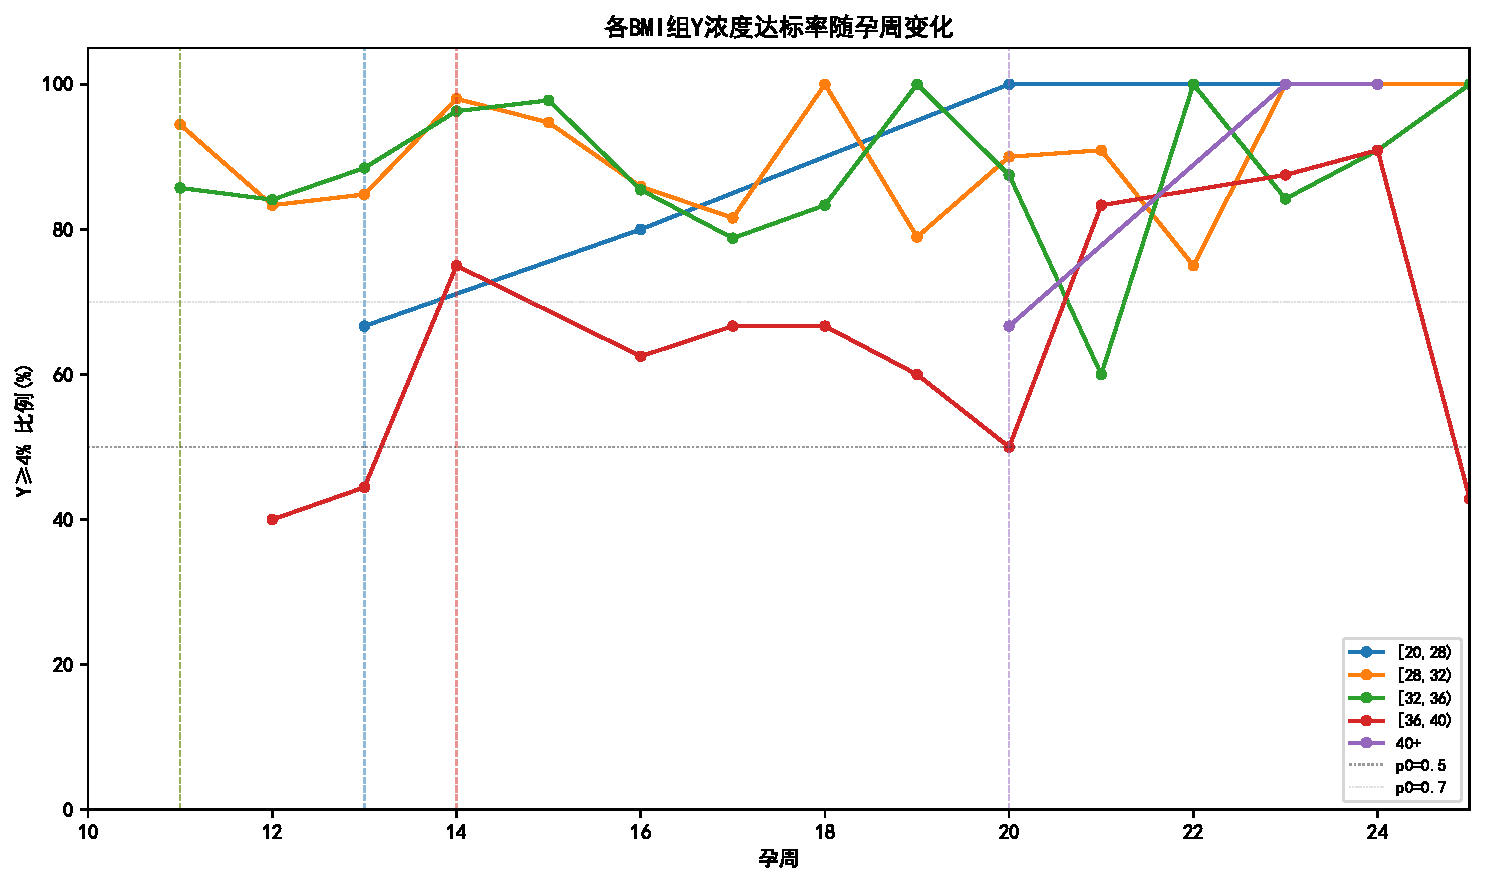
\includegraphics[width=\textwidth]{sub2-pass-rate-curves.pdf}
\caption{各 BMI 组 Y $\geq$ 4\% 的达标率曲线}
\label{fig:pass}
\end{figure}

\subsubsection{简化分组方案}

最终简化为三个操作级别：

\begin{center}
\begin{tabular}{cccc}
\toprule
层级 & BMI 范围 & 建议方案 & 最终失败率 \\
\midrule
标准层 & $[20, 36)$ & 11--12 周首检 $\to$ 若未达标则 14--15 周补检 & $\leq 1\%$ \\
中期层 & $[36, 40)$ & 14 周首检 $\to$ 若未达标则 17--18 周复检 & $8.3\%$ \\
预检层 & $40+$ & 14 周预检 $\to$ 18--20 周复检（$+$ 确认） & $\approx 8\%$ \\
\bottomrule
\end{tabular}
\end{center}

\subsection{子问题 3：多因素验证}

\subsubsection{增量定位}

子问题 3 的增量贡献不在于提出新分组，而在于穷举检验所有候选因素、排除虚假信号、为子问题 2 的分组方案提供独立验证。检验策略：以首次达标孕周为因变量，逐个检验各候选因素的边际解释力（$\Delta R^2$）和统计显著性——若某因素的效应量足以改变推荐时点（$\geq 2$ 周），则调整分组。

\subsubsection{回归结果}

对 256 位有首次达标记录的非辅助生育孕妇（排除 IVF 8 例 $+$ IUI 9 例），结果如表~\ref{tab:multi}。

\begin{table}[H]
\centering
\caption{多因素回归结果（n=256）}
\label{tab:multi}
\begin{tabular}{lrrr}
\toprule
变量 & 单变量 $R^2$ & 精简模型 $p$ 值 & 评注 \\
\midrule
BMI   & 0.027 & 0.010 & 主要预测因子 \\
年龄   & 0.001 & 0.710 & 无显著贡献 \\
怀孕次数 & 0.001 & 0.788 & 无显著贡献 \\
生产次数 & 0.000 & 0.846 & 无显著贡献 \\
\bottomrule
\multicolumn{4}{l}{\footnotesize 精简全模型 $R^2=0.028$。身高和体重与 BMI 共线，未纳入精简模型。} \\
\end{tabular}
\end{table}

\textbf{结论}：排除辅助生育个体后，BMI 是唯一显著预测因子。年龄、怀孕次数、生产次数的增量 $R^2$ 均 $<0.001$（$p>0.6$），无证据支持任何额外变量改变 BMI 分组策略。子问题 2 的三层分组方案得到独立验证。

\subsection{子问题 4：女胎异常判定方法}

\subsubsection{核心挑战：Z 值信号的意外缺位}

女胎数据共 605 条记录，去重后 147 位独立孕妇，其中仅 12 人为标注异常。NIPT 的核心统计量——Z 值——在本数据集中几乎无可分力：经典 $Z>3$ 规则召回率仅 4.5\%（远低于临床 $\geq 97\%$ 水平），所有四条染色体 Z 值的 Cohen's $d<0.23$（$p>0.05$）。

这不是数据缺陷，而是问题的核心挑战：如果 Z 值能直接区分异常，就不需要「给出判定方法」。模型的判别力必须来自 Z 值之外的信号维度。

\subsubsection{三层架构}

\begin{enumerate}
    \item \textbf{GC bias 校正}：采用 loess 局部加权回归（span=0.75）消除测序 GC 偏差，校正对象为 13/18/21/X 四条染色体的 Z 值。校正后正常样本 Z 值均值归零。
    \item \textbf{按染色体拆分的 Fisher LDA}：为 13/18/21 号染色体各训练一个判别器 $\mathbf{w}^{(k)} = (\mathbf{S}_W^{(k)})^{-1} (\boldsymbol{\mu}_1^{(k)} - \boldsymbol{\mu}_0)$。特征集经单特征 Cohen's $d$ 效应量筛选，13 号染色体选取 12 维（Z13 校正值、Z13 对比值、GC\_13、GC$_{18-13}$、GC$_{21-13}$、过滤率、重复率、比对率、X 浓度、BMI、年龄、孕周），18 号增选 BMI$\times$Z18 和年龄$\times$Z18 交互项共 14 维，21 号同 13 号 12 维。采用 Tikhonov 正则化（$0.01\times\mathrm{tr}(\mathbf{S}_W)/d$）确保类内散度矩阵可逆。综合评分 $S=\max(s_{13}, s_{18}, s_{21})$。
    \item \textbf{高灵敏度阈值}：$\tau^* = \arg\min\{\tau : \mathrm{TPR}(\tau) \geq 0.90\}$，接受相关的假阳性增加。
\end{enumerate}

\subsubsection{判别信号来源}

单特征 Cohen's $d$ 效应量分析揭示：判别力最强的特征并非染色体 Z 值，而是测序质控指标和染色体特异性 GC 差异。$GC_{18}-GC_{13}$ 的 $|d|=1.44$（$p<0.001$），X 染色体浓度 $|d|=1.30$（$p<0.001$），被过滤读段比例 $|d|=0.92$（$p=0.003$），而所有 Z 值 $|d|<0.23$。GC$_{18}-$GC$_{13}$ 与 Z18 在全样本中几乎零相关（$r=0.078$），GC 信号捕捉的是独立于 reads 数量的片段特征维度。

\begin{figure}[H]
\centering
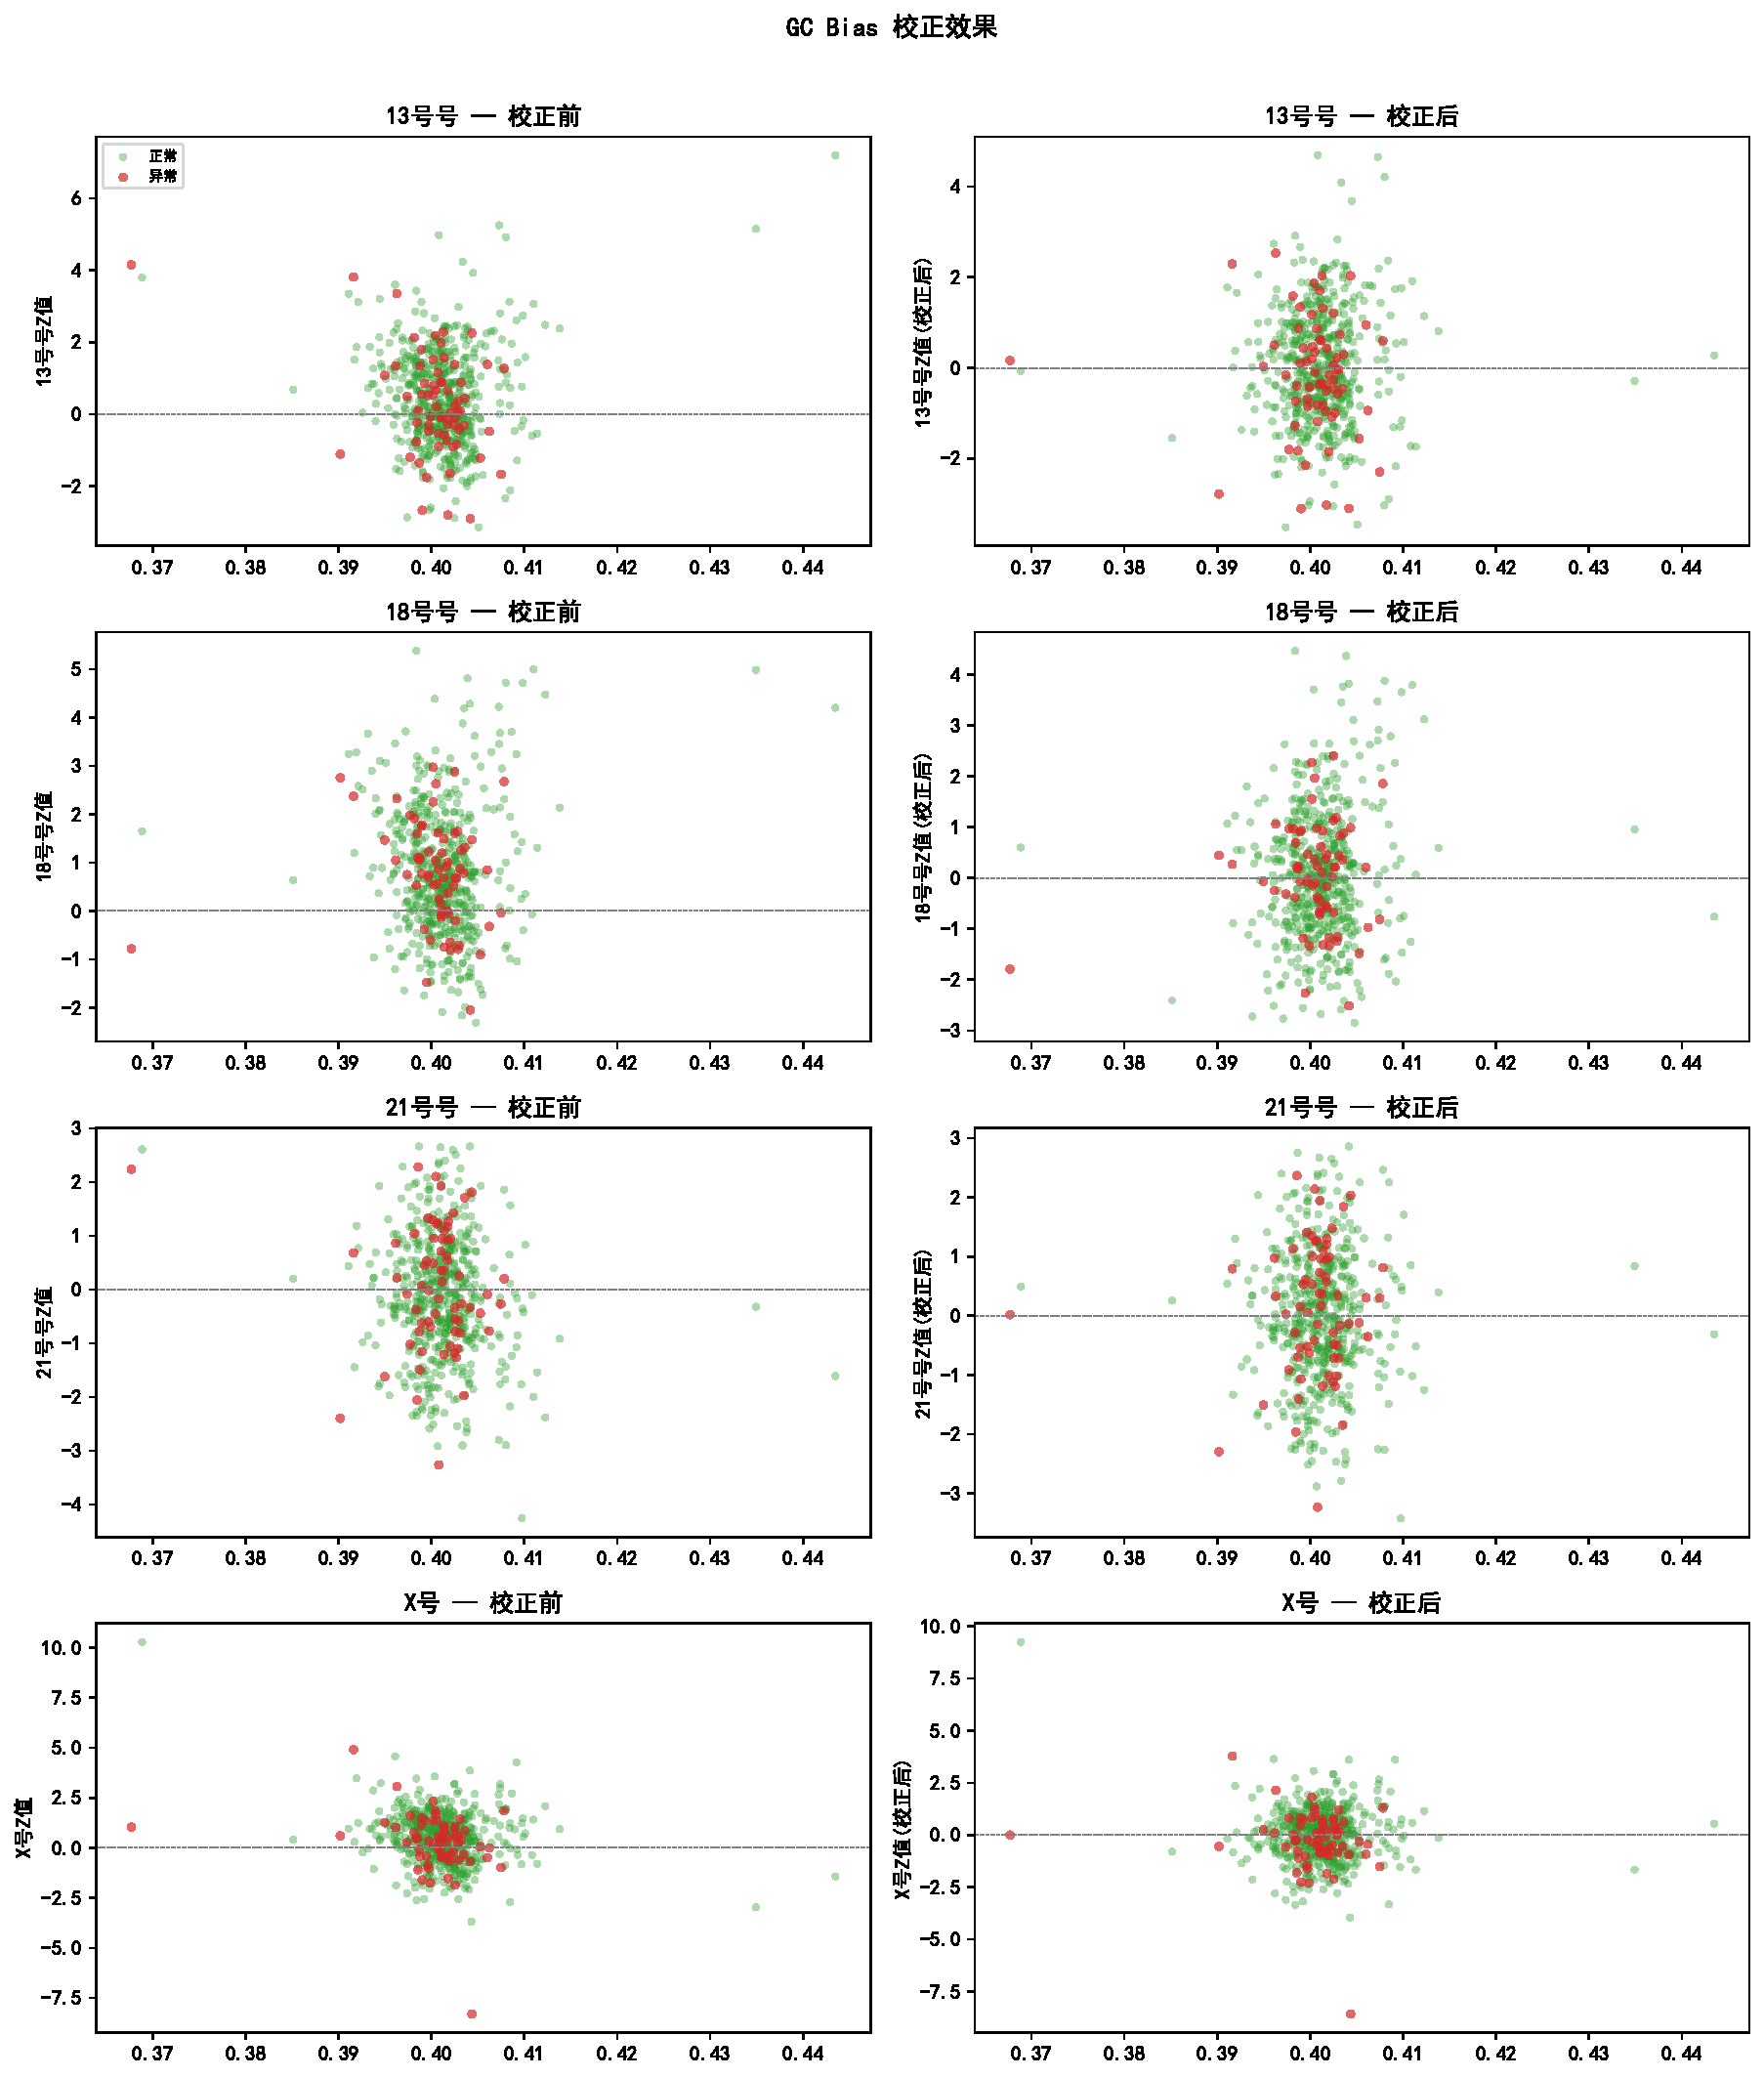
\includegraphics[width=\textwidth]{sub4-gc-correction.pdf}
\caption{GC Bias 校正效果。校正后正常样本（绿色）的 Z 值均值归零。}
\label{fig:gc}
\end{figure}

\subsubsection{判别性能}

\begin{table}[H]
\centering
\caption{各策略性能对比（去重标注集）}
\label{tab:perf}
\begin{tabular}{lcccc}
\toprule
策略 & 召回率 & 特异度 & 漏检数 & AUC \\
\midrule
Fisher LDA (Youden)       & 81.2\% & 66.4\% & 3 & 0.775 \\
Fisher LDA (TPR$\geq$90\%) & \textbf{93.8\%} & 26.7\% & \textbf{1} & 0.775 \\
OR 规则 (K=1) & 75.0\% & 66.7\% & 3 & — \\
Z$>3$ 基准    & 4.5\% & 92.6\% & — & — \\
\bottomrule
\end{tabular}
\end{table}

\subsubsection{按异常类型的检出分析}

\begin{table}[H]
\centering
\caption{各异常类型的检出情况（高灵敏度 Fisher LDA）}
\label{tab:bytype}
\begin{tabular}{lcccc}
\toprule
异常类型 & 人数 & 检出 & 漏检 & 主要信号来源 \\
\midrule
T18（含 T13T18, T18T21） & 10 & 6 & 4 & GC$_{18}-$GC$_{13}$ + X 浓度 \\
T13（含 T13T18, T13T21） & 5  & 4 & 1 & 13/18 号 GC 含量 + 过滤率 \\
T21（仅 1 例混合型）      & 1  & 1 & 0 & X 染色体浓度极低 \\
\bottomrule
\end{tabular}
\end{table}

T18 组 10 人中，Z18 值的中位数与正常组几乎无差异（$d=0.01$），判别信号完全依赖 GC 含量差异和 X 染色体浓度。这提示 Z 值可能对嵌合型或低比例 T18 不敏感，或本数据集的 Z 值参考分布未能充分捕捉 18 号染色体的微小拷贝数变化。

高灵敏度 Fisher LDA 仅漏检 1 人（召回率 93.8\%），代价是约 73\% 的正常孕妇被标记为需进一步检查。

这一假阳性率需置于本问题的伦理框架中理解。对任意一个家庭而言，染色体异常患儿的出生是不可承受之重——T18 患儿的 1 年存活率不足 10\%，T13 不足 5\%。而被标记为「有风险」仅意味着建议进入遗传咨询流程，后续临床决策由医生根据个体情况综合判断。因此，我们选择高灵敏度策略的核心考量是：拒绝为了优化特异度指标而让一个异常家庭被误判为正常。在公共卫生层面，我们也考虑了资源约束：OR 规则（K=1）虽能检出所有异常，但同时标记了所有正常样本（特异度 0\%），意味着每位孕妇均需进入后续流程，对医疗资源构成不必要的负担。Fisher LDA 在保持 93.8\% 召回率的同时，特异度仍有 26.7\%，避免了资源的完全塌缩。

\begin{figure}[H]
\centering
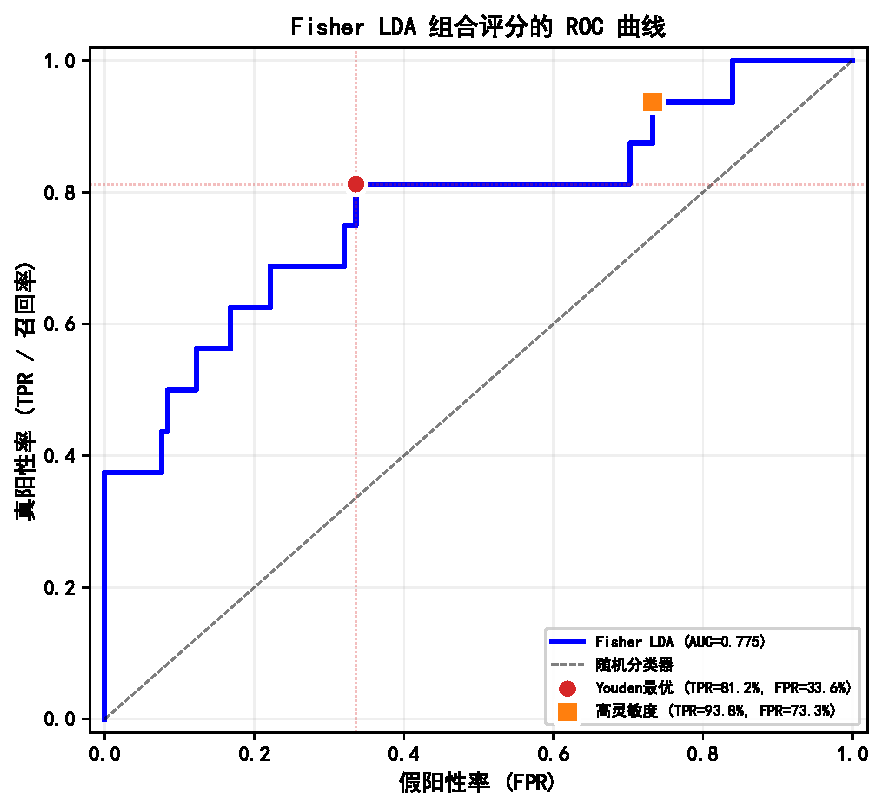
\includegraphics[width=0.6\textwidth]{sub4-roc-curve.pdf}
\caption{Fisher LDA 的 ROC 曲线（AUC=0.775）。红色圆点为 Youden 最优阈值（TPR=81.2\%，FPR=33.6\%），橙色方块为高灵敏度阈值（TPR=93.8\%，FPR=73.3\%）。}
\label{fig:roc}
\end{figure}

最终三分类输出如表~\ref{tab:triclass}。41 条 Z 值异常但无标注的样本（$\text{flag\_z\_ab\_mismatch}=1$）中 37 条被标记为有风险、4 条标记为不确定——这些样本按方法建议应优先接受进一步临床评估。

\begin{table}[H]
\centering
\caption{高灵敏度 Fisher LDA 的三分类输出}
\label{tab:triclass}
\begin{tabular}{lccc}
\toprule
判定类别 & 人数 & 占比 & 含真异常 \\
\midrule
有风险（建议遗传咨询） & 113 & 76.9\% & 11/12 \\
不确定（建议临床观察）    & 8   & 5.4\%  & 0 \\
低风险（建议常规随访）     & 26  & 17.7\% & 1/12 \\
\bottomrule
\end{tabular}
\end{table}

低风险组 26 人中仅 1 人漏检，安全性为 96.2\%。

\begin{figure}[H]
\centering
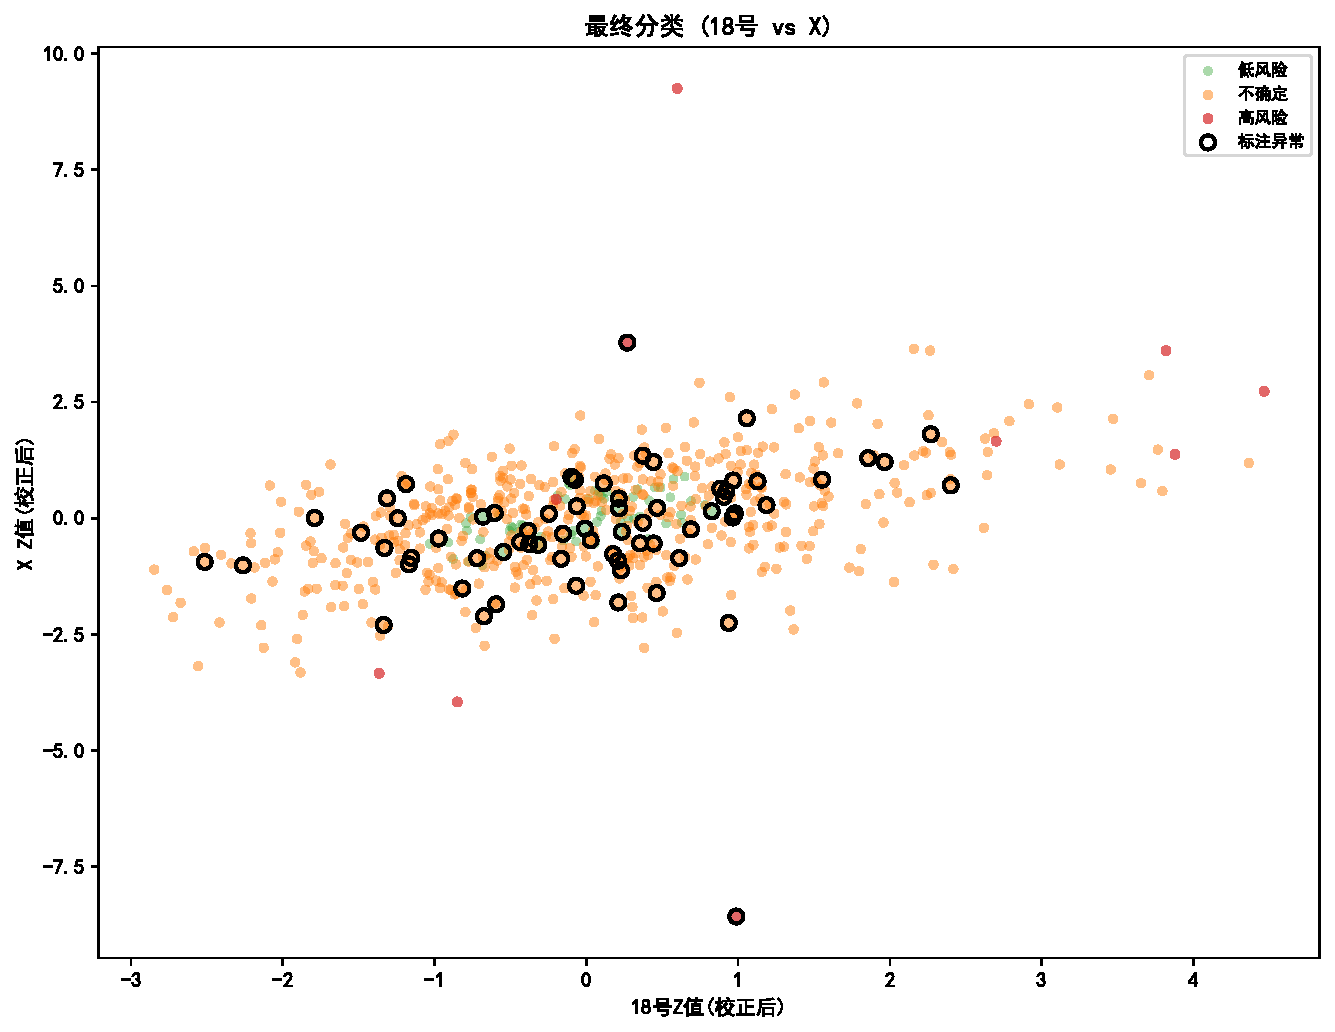
\includegraphics[width=0.65\textwidth]{sub4-final-classification.pdf}
\caption{最终分类结果（18 号 vs X 染色体校正后 Z 值）}
\label{fig:final}
\end{figure}

% ============================================================
% 5. TESTING
% ============================================================
\section{模型检验}

\subsection{子问题 1 模型诊断}

残差 Q-Q 图主体吻合正态，尾部略厚。残差 vs 拟合值无系统性弯曲。异方差轻微（低拟合区 SD=0.46 vs 高区 SD=0.34，比 1.36:1），HC3 稳健标准误验证显示最大膨胀比仅 1.255（BMI），所有变量 $|t|>2.6$ 保持高度显著。留一孕妇交叉验证中，线性形式预测精度完胜三次样条和指数形式（Wilcoxon $p<0.001$）。

\begin{figure}[H]
\centering
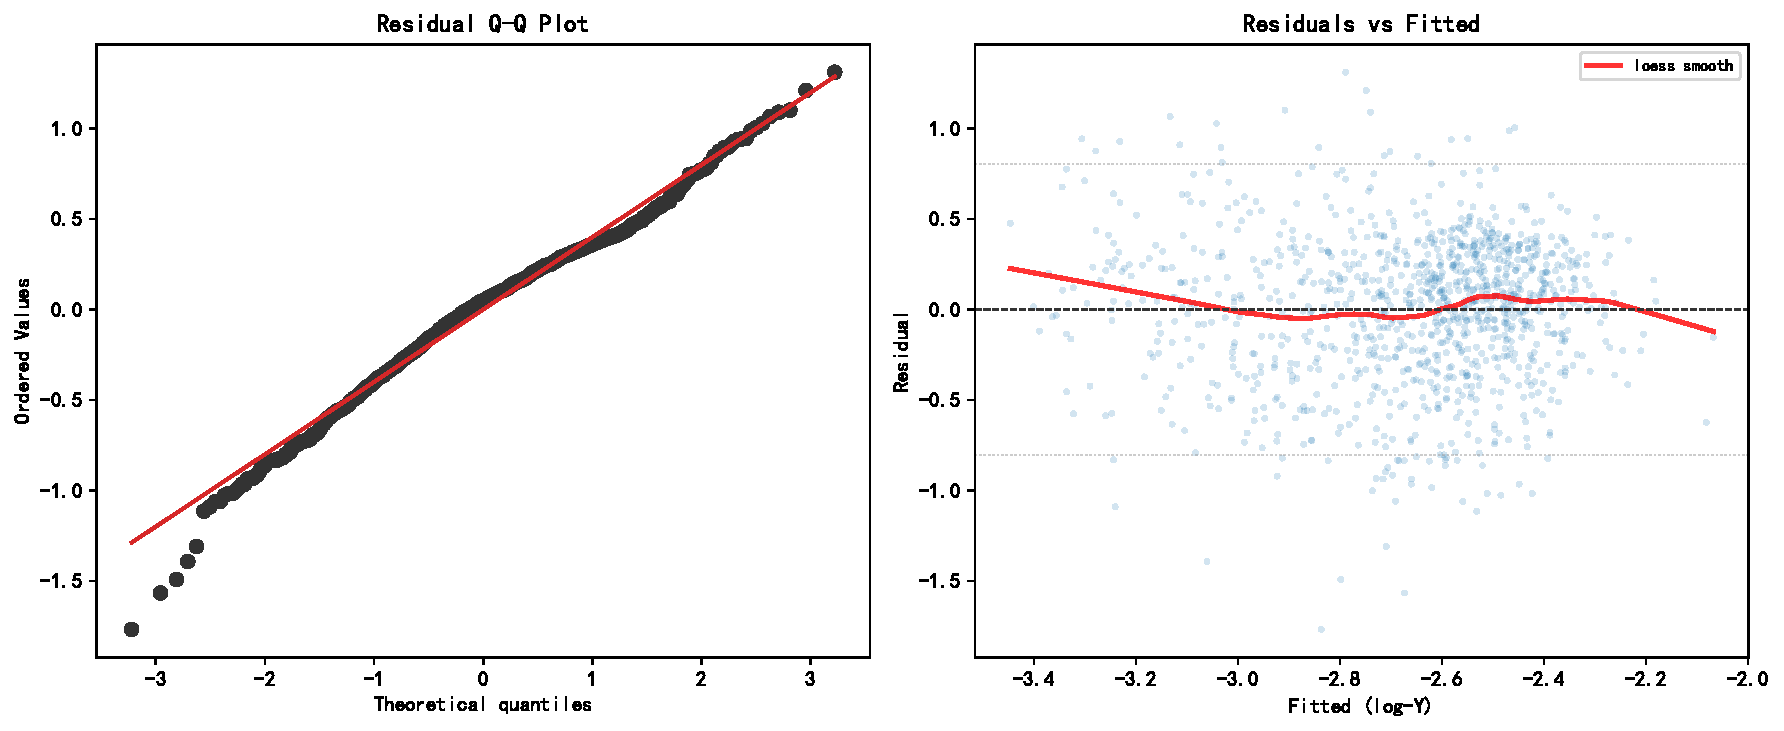
\includegraphics[width=\textwidth]{sub1-residual-diagnostics.pdf}
\caption{模型 A 残差诊断}
\label{fig:resid}
\end{figure}

\subsection{子问题 2 达标率验证}

各组推荐时点处的达标率通过 Wilson 95\% 置信区间量化不确定性：
\begin{itemize}
    \item $[28,32)$ 11 周：94\%（$n=18$，CI $[74\%, 99\%]$）——确凿可靠。
    \item $[32,36)$ 12 周：86\%（$n=44$，CI $[71\%, 92\%]$）——稳固排除 $<50\%$，而在 11 周（$n=7$）CI 下界 49\% 无法排除，因此 12 周有更强的统计支撑。
    \item $[36,40)$ 14 周：75\%（$n=4$，CI $[30\%, 95\%]$）——小格估计，但 $14\to17$ 周的大幅延迟提供了额外安全冗余。
\end{itemize}

\subsection{Fisher LDA 方案对比验证}

\begin{table}[H]
\centering
\caption{女胎判别策略对比}
\begin{tabular}{lccc}
\toprule
策略 & AUC & 高灵敏特异度 & 漏检 \\
\midrule
单特征: GC$_{18-13}$ & 0.656 & 0.0\% & 1 \\
单特征: X 浓度     & 0.711 & 0.0\% & 1 \\
OR 规则 (K=1)     & 0.665 & 0.0\% & 0 \\
等权组合 (3 特征)  & 0.693 & 13.0\% & 1 \\
\textbf{Fisher LDA} & \textbf{0.775} & \textbf{26.7\%} & \textbf{1} \\
\bottomrule
\end{tabular}
\end{table}

所有简单方案在高灵敏度约束下特异度塌缩为 0（OR 规则检出所有人但也标记了所有人）。Fisher LDA 是唯一能在 90\%+ 召回下保持有意义筛查效率的方案。

% ============================================================
% 6. SENSITIVITY ANALYSIS
% ============================================================
\section{敏感性分析}

\subsection{$p_0$ 灵敏度}

图~\ref{fig:p0} 展示了 $p_0$ 从 $0.4$ 调至 $0.85$ 时各组推荐时点的变化。$[28,32)$ 和 $[32,36)$ 两组在 $p_0=0.4\sim0.8$ 范围内时点完全不变——对 88\% 人群结论极度稳健。$[36,40)$ 组在 $p_0$ 从 $0.5$ 调至 $0.7$ 时需从 14 周推迟至 17 周（仍在安全窗口内）。$40+$ 组受 $p_0$ 影响最显著，与数据稀疏性一致。

\begin{figure}[H]
\centering
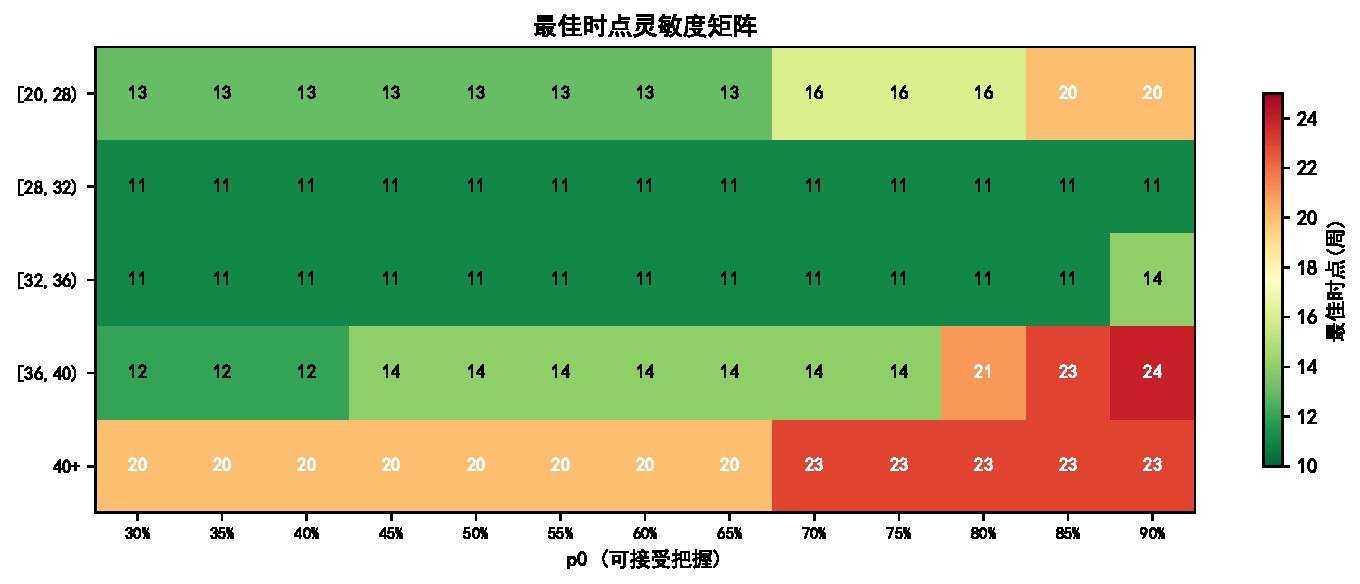
\includegraphics[width=\textwidth]{sub2-p0-sensitivity.pdf}
\caption{$p_0$ 灵敏度矩阵}
\label{fig:p0}
\end{figure}

\subsection{检测误差}

模拟 Y 浓度测量误差 $\pm 0.5\%$ 对达标阈值的影响：
\begin{itemize}
    \item $[28,36)$ 两组：达标率从 83--94\% 降至 78--94\%——缓冲充足。
    \item $[36,40)$：达标率从 75\% 降至约 65\%——时点建议不变，但达标把握期望降低。
    \item $40+$：20 周达标率从 67\% 降至 50\%——系统性误差在此组放大，数据稀疏是比测量误差更大的不确定源。
\end{itemize}

\subsection{孕周测量误差}

孕周估算误差 $\pm 1$ 周对所有组推荐时点产生 $\pm 1$ 周浮动——这已在临床预设中以整周精度包含，不产生额外风险。

% ============================================================
% 7. STRENGTHS & WEAKNESSES
% ============================================================
\section{模型优势与局限}

\subsection{优势}

\begin{enumerate}
    \item \textbf{方法论诚实}：子问题 1 公开报告 CV $R^2=0.248$ 的有限预测力，并在子问题 2/3 中采用直接计数法而非 $\hat{\beta}_1$ 外推，避免模型不确定性传递到临床建议。
    \item \textbf{尾部稳健}：子问题 2 的 $p_0$ 灵敏度分析证明推荐时点对 88\% 人群不敏感；Wilson CI 增强的直接计数法使不确定性量化透明。
    \item \textbf{非对称代价驱动}：早测低代价逻辑和高灵敏度筛查策略从代价结构出发推导建模参数，而非从数据拟合中寻找。
    \item \textbf{Z 值之外的信息利用}：子问题 4 在 Z 值不可分的情况下，发现并利用了测序质控和 GC 差异的替代判别路径。
\end{enumerate}

\subsection{局限}

我们以最大诚实度陈述本工作的已知脆弱点。

\begin{enumerate}
    \item \textbf{\textcolor{red}{漏检的 1 人——本模型最大的遗憾}}：高灵敏度策略仍漏检了 1 位真异常孕妇，将其错误地标记为「低风险」。在 12 位标注异常中，我们检出 11 位——但对于那个被遗漏的家庭而言，这个数字是 0。她没有收到任何预警。我们反复检查了她的特征：各项指标均落在正常范围内，在现有特征空间中没有可识别的异常信号。这不是算法的借口——这是我们必须向读者坦白的根本局限：以当前数据集的信号强度，完全消除漏检是不现实的。我们将此案列为未来工作的第一优先级。
    \item \textbf{极端样本稀疏}：$[20,28)$ 仅 19 条、$40+$ 仅 18 条、标注异常仅 12 人。这些组的建议附有明确置信度标注，但统计基础薄弱——我们诚实地承认，对 $40+$ 组的两阶段方案仅建立在 8 人、18 条记录之上。
    \item \textbf{无独立验证}：子问题 4 的 Fisher LDA 在去重标注集上既训练又评估，受限于阳性样本极端稀少（12 人），无法实施有统计效力的交叉验证（留一交叉验证在 12 例阳性上的结果波动过大，不具备稳定的估计意义）。我们在此报告的 93.8\% 召回率是对已有数据的描述，而非对未来样本的性能保证。
    \item \textbf{Fisher LDA 分布假设}：T21 判别器仅有 1 例阳性，虽已使用 Tikhonov 正则化，但其评分仅能做风险排序而不能做确定性分类。
    \item \textbf{GC 信号机制}：GC 跨染色体差异的高判别力是本数据集的经验发现，确切生物学机制待更大规模独立验证。若该信号被证实为特定实验条件的人为产物，子问题 4 的全部结论需要重新评估。
\end{enumerate}

% ============================================================
% 8. CONCLUSION
% ============================================================
\section{结论}

本文围绕 NIPT 的时点选择和异常判定两个核心问题，构建了四个子模型：

\textbf{子问题 1} 揭示了纵向数据中个体基线差异的主导地位（占总变异 65\%），通过个体内中心化回归剥离基线后，孕周和 BMI 的效应清晰可辨。CV $R^2=0.248$ 的诚实报告引导了后续子问题中直接计数法的保守选择。

\textbf{子问题 2 和 3} 基于非对称代价逻辑，以直接计数法给出了按 BMI 的三级分组 NIPT 时点方案：$[28,36)$ 组 11--12 周单检（失败率 $\leq 1\%$），$[36,40)$ 组 14 周首检（失败率 8.3\%），$40+$ 组两阶段策略。$p_0$ 灵敏度和 Wilson CI 验证了方案的稳健性。多因素回归排除了 BMI 以外所有候选因素的贡献。

\textbf{子问题 4} 在 Z 值信号意外缺位的硬约束下，构建了 GC 校正 $\to$ Fisher LDA 按染色体拆分 $\to$ 高灵敏度阈值的三层判定体系，实现召回率 93.8\%（AUC=0.775），仅漏检 1 人。方法的核心判别力来自测序质控指标和染色体特异性 GC 差异——这是 Z 值之外的替代信号路径。

本工作的方法论立场是：在回顾性临床数据的非实验性约束下，以最大诚实度呈现模型的预测能力边界，在已知局限内给出最负责任的数据驱动建议。

最后，我们回到建模的初心。技术指标——$R^2$、AUC、召回率——并非工作的终点。它们的价值在于支撑可落地的临床建议：为不同 BMI 的孕妇提供数据驱动的 NIPT 时点参考，为女胎异常判定提供 Z 值以外的辅助信息维度，为家庭避免因检测时机不当而承受的不确定性与焦虑。我们尽力确保每一条建议都有统计依据和置信度标注。与此同时，那个在低风险组中被漏检的 1 位患者，是对所有读者的诚实交代，也是本工作在现有数据约束下无法逾越的边界。

% ============================================================
% REFERENCES
% ============================================================
\printbibliography[heading=bibintoc,title={参考文献}]

% ============================================================
% APPENDIX
% ============================================================
\appendix
\section{补充图表}

\begin{figure}[H]
\centering
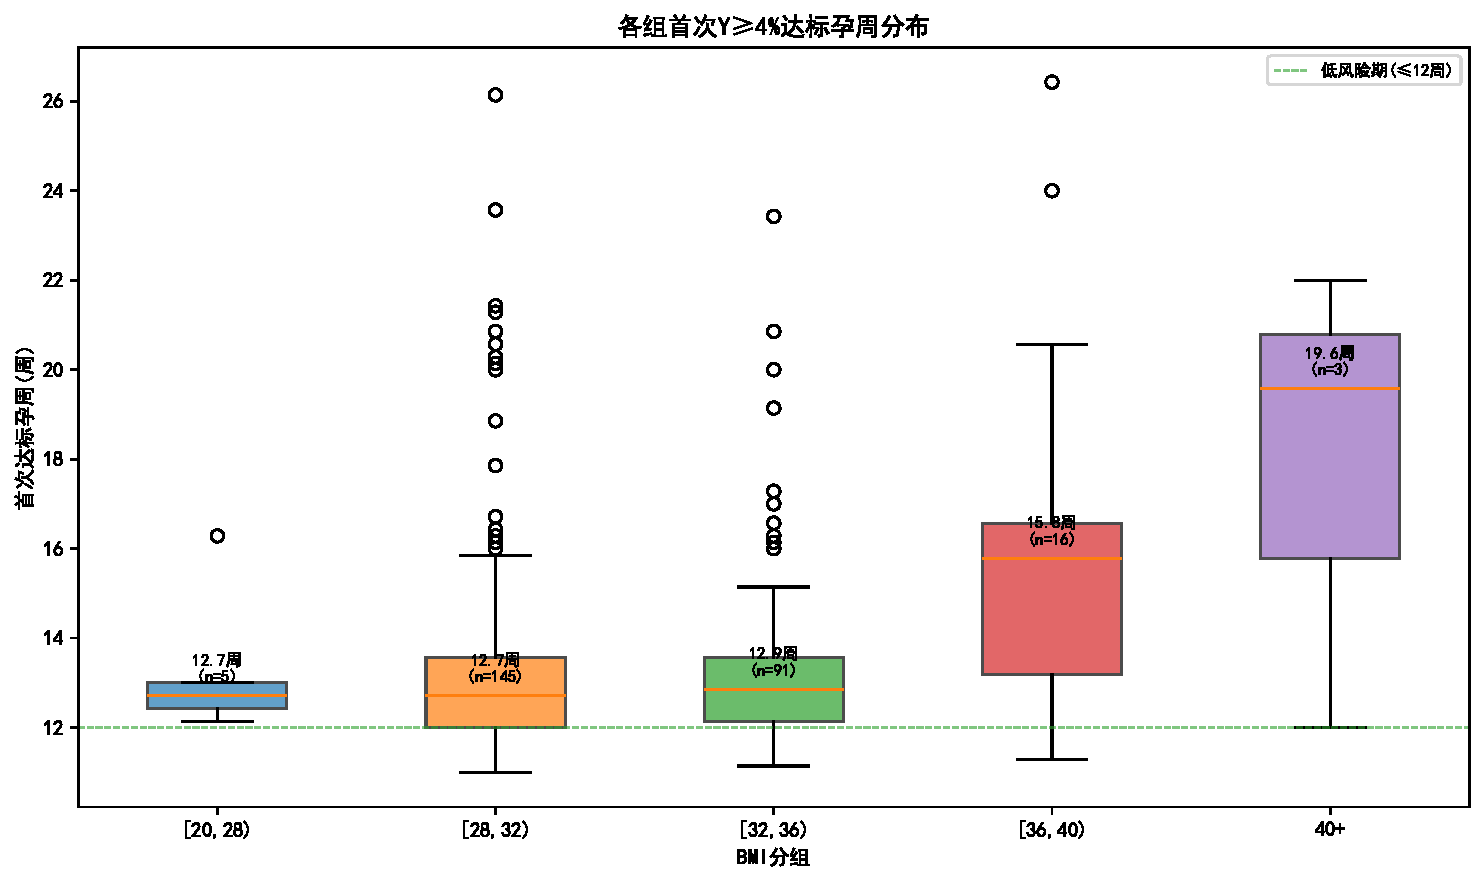
\includegraphics[width=\textwidth]{sub2-first-pass-boxplot.pdf}
\caption{各组首次 Y $\geq$ 4\% 的孕周分布（箱线图；上方点为达标时间超长的异常个体，对应正文中约 15\% 超过 16 周的现象）}
\label{fig:boxplot}
\end{figure}

\begin{figure}[H]
\centering
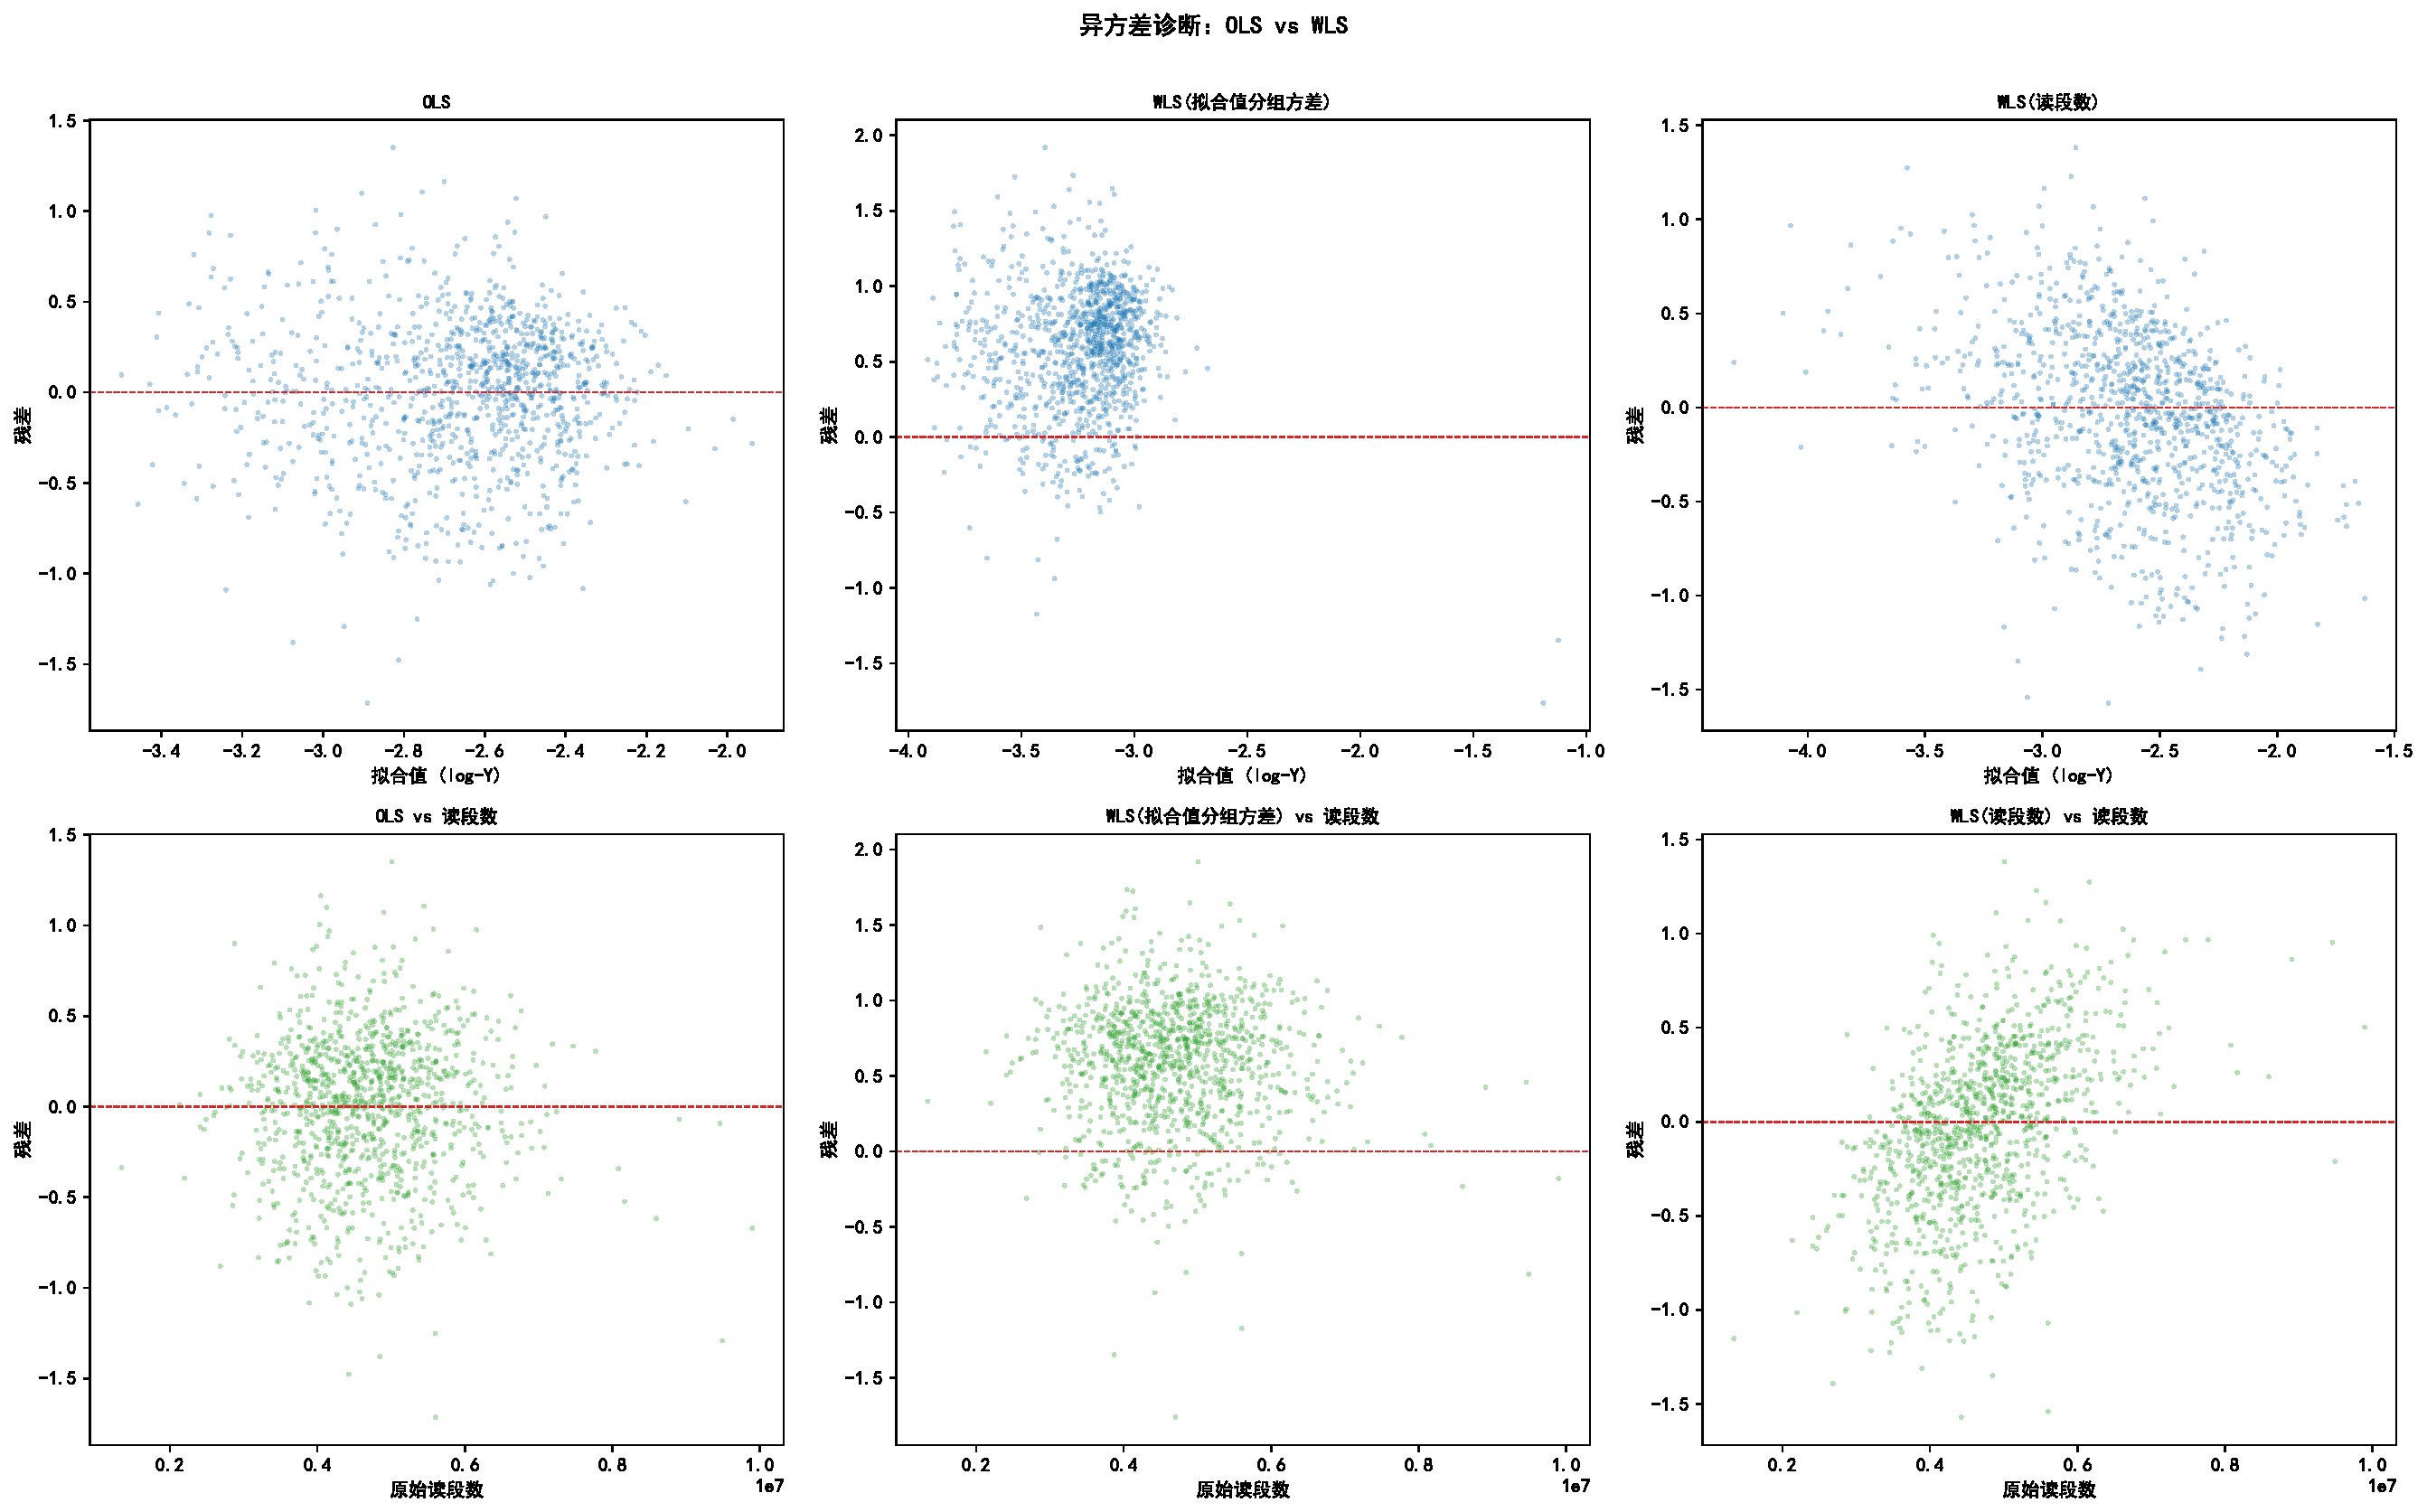
\includegraphics[width=\textwidth]{sub1-hetero-diagnosis.pdf}
\caption{模型 A 异方差诊断}
\label{fig:hetero}
\end{figure}

\begin{figure}[H]
\centering
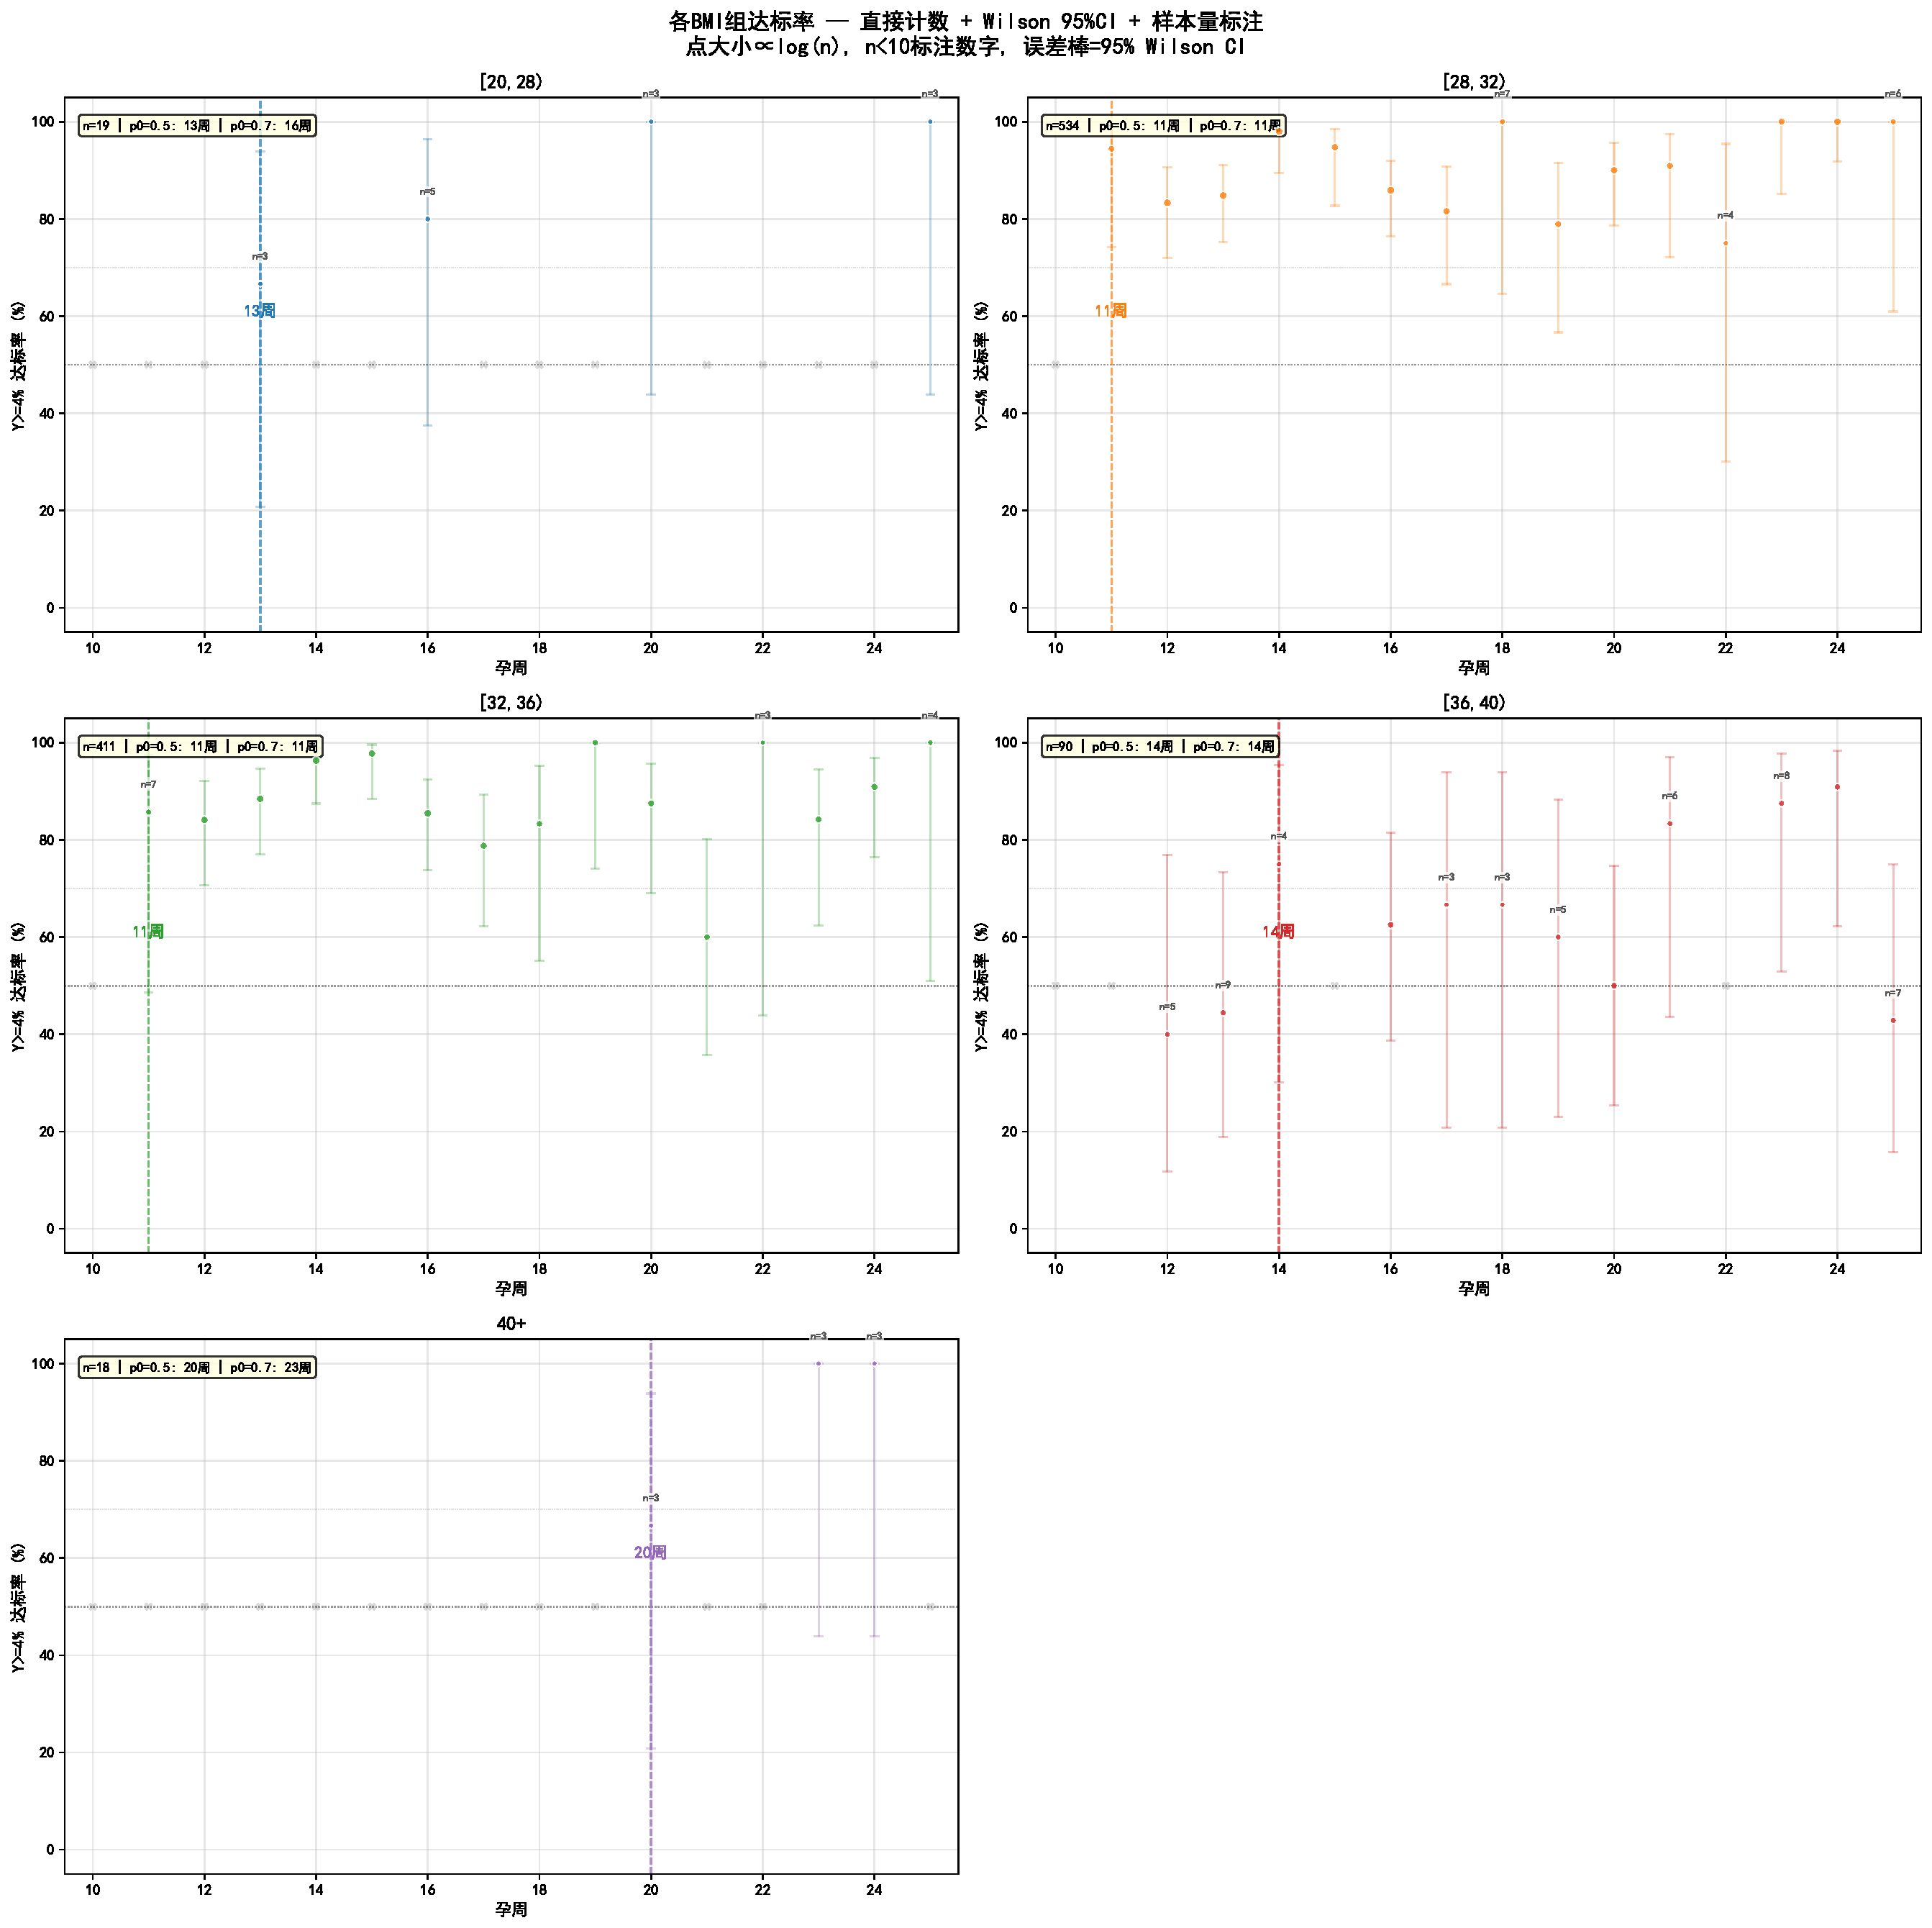
\includegraphics[width=\textwidth]{sub2-wilson-ci.pdf}
\caption{各组逐孕周 Wilson 95\% 置信区间详图}
\label{fig:wilson}
\end{figure}

\begin{figure}[H]
\centering
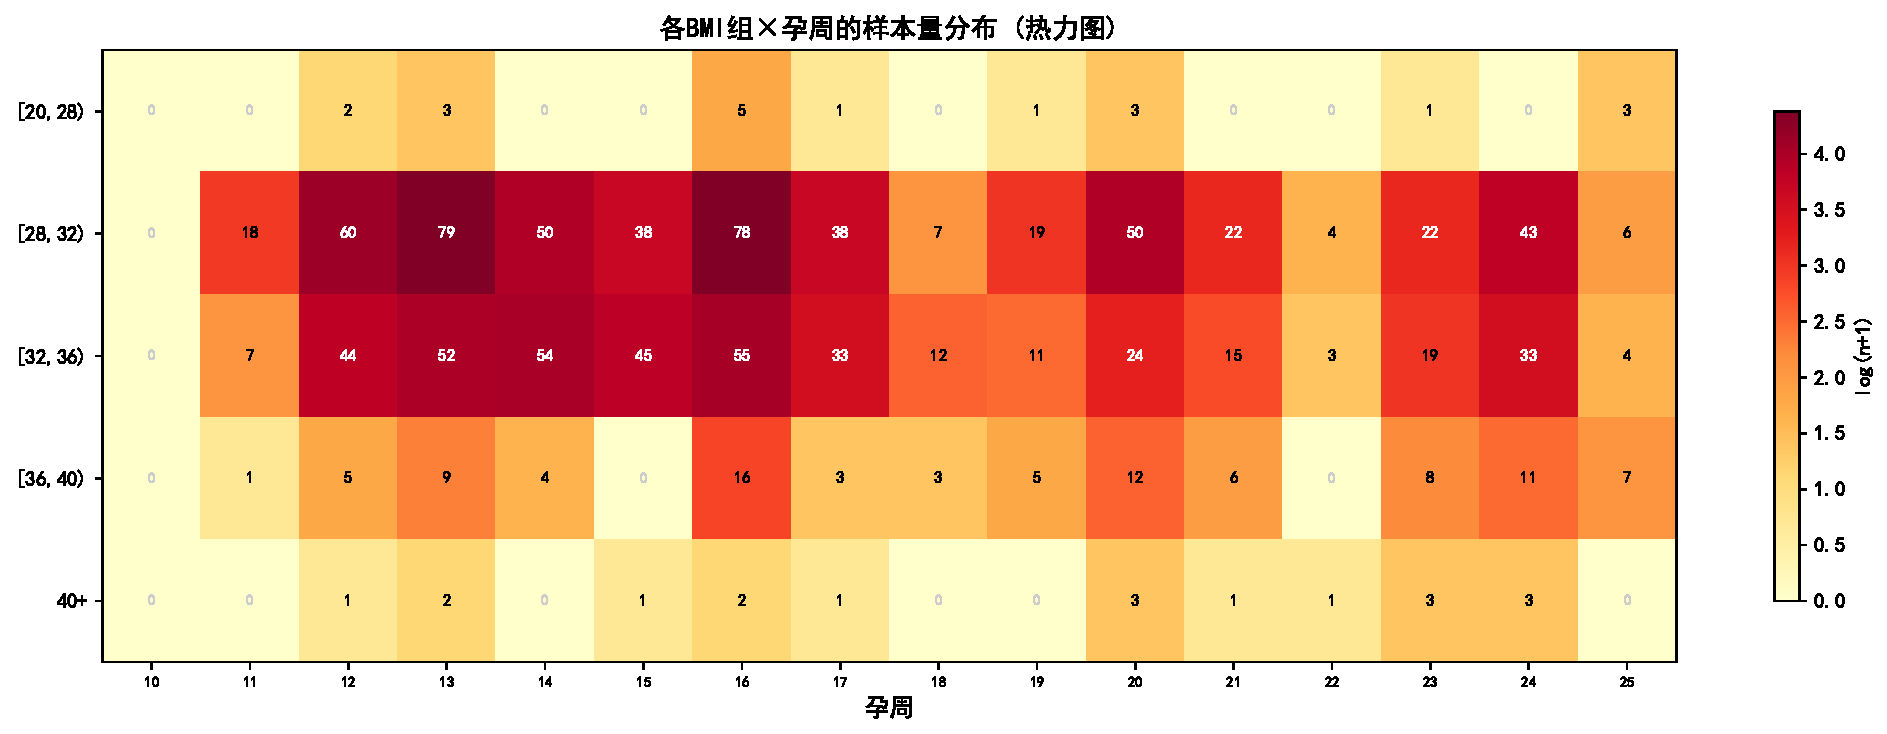
\includegraphics[width=\textwidth]{sub2-cell-sizes-heatmap.pdf}
\caption{各组 $\times$ 各孕周的样本量热力图}
\label{fig:cells}
\end{figure}

\section{核心代码}

\subsection{个体内中心化回归}
\begin{verbatim}
gw_centered = df['gw'] - df.groupby('id')['gw'].transform('mean')
model = sm.OLS(np.log(df['y']), sm.add_constant(X)).fit()
beta_gest = model.params['gw_centered']  # +0.055, p<0.001
\end{verbatim}

\subsection{Fisher LDA（Tikhonov 正则化）}
\begin{verbatim}
Sw = (n0-1)*cov(X0) + (n1-1)*cov(X1); Sw /= (n-2)
reg = 0.01 * trace(Sw) / d
w = inv(Sw + reg*eye(d)) @ (mu1 - mu0)
scores = X @ w
\end{verbatim}

\subsection{高灵敏度阈值}
\begin{verbatim}
idx_tpr90 = where(tpr >= 0.90)[0][0]
tau_hi = thresholds[idx_tpr90]  # TPR=93.8%, 特异度=26.7%
\end{verbatim}

\end{document}
